\PassOptionsToPackage{natbib}{biblatex}
\documentclass{bredele}
\addbibresource{references.bib}

\usepackage{makecell, amssymb, amsthm, mathtools, rotating, colortbl, enumitem, nomencl, latexsym, bookmark, url, subcaption, float, multirow, algorithm, algorithmic, color}
\usepackage{arabtex, utf8}
\setcode{utf8}
\usepackage[nomain, acronym]{glossaries}

\makeglossaries


\definecolor{Skyblue}{rgb}{0.15,0.4,0.65}

\floatstyle{plaintop}
\restylefloat{table}

\newtheoremstyle{mystyle}%             % Name
{}%                                    % Space above
{}%                                    % Space below
{\itshape}%                            % Body font
{}%                                    % Indent amount
{\bfseries}%                           % Theorem head font
{}%                                    % Punctuation after theorem head
{\newline}%                            % Space after theorem head, ' ', or \newline
{}%                                    % Theorem head spec (can be left empty, meaning `normal')

\theoremstyle{mystyle}

\addto\captionsfrench{\def\tablename{Tableau}}
\setlist[itemize]{label=\textbullet}
\setcounter{secnumdepth}{3}

\pagenumbering{Roman}

\makeatletter
\newcommand{\closenomencl}{%
	\closeout\@nomenclaturefile%
}
\makeatother

\newcommand{\writenomencl}[1]{%
	\closenomencl%
	\IfFileExists{#1.nlo}{%
		\write18{%
			makeindex -s nomencl.ist -o #1.nls -t #1.nlg #1.nlo%
		}% 
	}{\typeout{Nothing there}}%
}

\AtEndDocument{\writenomencl{\jobname}}

% Remove " CHAPTER 0 " from header
\renewcommand{\chaptermark}[1]{%
	\ifnum\value{chapter}>0
	\markboth{Chapitre \thechapter{}: #1}{}%
	\else
	\markboth{#1}{}%
	\fi}

\title{\textbf{\textcolor{Skyblue}{Conception et simulation d'un système d'échange de clés S-SEJAD}}}

\discipline{Informatique}

\jury{
	\begin{description}		
		\item[Président~:]~~~~~~~~~~~~~~ Hamidou \textsc{Dathe}, Professeur, Université Cheikh Anta Diop
		\item[Rapporteurs~:]~~~~~~~~~ .... \textsc{....}, .................................
		\item[]~~~~~~~~~~~~~~~~~~~~~~~~~~~~~~ ....  \textsc{....}, .................................	
		\item[Examinateurs~:]~~~~~~~ .... \textsc{....}, .................................
		\item[]~~~~~~~~~~~~~~~~~~~~~~~~~~~~~~ .... \textsc{....}, .................................
		\item[Co-endadrant~:]\ Khadidiatou   \textsc{WANE Keita},Maître de Conférences , Université Cheikh Anta Diop
		\item[Directeur de thèse~:]\ Khaly  \textsc{TALL}, Professeur, Université Cheikh Anta Diop
	\end{description}
}

\logouniversite{Images/ISCAE}
\scalelogouniversite{0.3}

\unite{\large Présenté par\\ Mohamed Saleck Lebchir}
\ecoledoc{Pour obtenir le diplôme de\\Master Professionnel de l'ISCAE}


\begin{document}
	
	\maketitle
	
	\tableofcontents
	\listoffigures
	\let\cleardoublepage\clearpage
	\listoftables
	
	\newacronym{UML}{UML}{Unified Modeling Language.}
	\newacronym{API}{API}{Application Programming Interface.}
	\newacronym{DAO}{DAO}{Data Access Object.}
	\newacronym{IDE}{IDE}{Integrated Development Environment (Environnement de Développement Intégré).}
	\newacronym{HTTP}{HTTP}{HyperText Transfer Protocol.}
	\newacronym{HTTPS}{HTTPS}{HyperText Transfer Protocol Secure.}
	\newacronym{JSON}{JSON}{JavaScript Object Notation.}
	\newacronym{MERISE}{MERISE}{Méthode d’Étude et de Réalisation Informatique par les Sous-Ensembles ou pour les Systèmes d’Entreprise.}
	\newacronym{MVC}{MVC}{Model-View-Controller.}
	\newacronym{SGBD}{SGBD}{Système de Gestion de Bases de Données.}
	\newacronym{SGBDR}{SGBDR}{Système de Gestion de Bases de Données Relationnelle.}
	\newacronym{OTP}{OPT}{One-Time Password}
	\newacronym{SOA}{SOA}{Service Oriented Architecture}
	\newacronym{ORM}{ORM}{Object-Relational Mapping (en français Mapping Objet-Relationnel)}
	\newacronym{APK}{APK}{Android Package Kit}
	\newacronym{AAB}{AAB}{Android App Bundles}
	
	\printacronyms
	\printglossary[title={List of Abbreviations}]

	\let\cleardoublepage\clearpage

\chapter{Introduction générale}
\label{sec:DescriptionDuProjet}

Savoir qui est votre client et adopter des protocoles pour prévenir la criminalité financière sont des défis permanents pour les institutions financières. De manière significative, les institutions financières (y compris les banques, les coopératives de crédit et les sociétés financières du Fortune 50) doivent se conformer à un ensemble de réglementations de plus en plus complexes pour la vérification de l'identité des clients appelée KYC.

KYC, également connu sous le nom de "Know Your Customer" ou "Know Your Client", est un ensemble de procédures permettant de vérifier l'identité d'un client avant ou pendant les transactions avec les banques et autres institutions financières. Le respect des réglementations KYC peut aider à tenir à distance le blanchiment d'argent, le financement du terrorisme et d'autres stratagèmes de fraude courants. En vérifiant d'abord l'identité et les intentions d'un client au moment de l'ouverture du compte, puis en comprenant ses habitudes de transaction, les institutions financières sont en mesure d'identifier plus précisément les activités suspectes. 

Les institutions financières sont soumises à des normes de plus en plus strictes en matière de lois KYC. Ils doivent dépenser plus d'argent pour se conformer à KYC ou être passibles de lourdes amendes. Ces réglementations signifient que presque toutes les entreprises, plateformes ou organisations qui interagissent avec une institution financière pour ouvrir un compte ou effectuer des transactions devront se conformer à ces obligations.

La gestion de la relation client (CRM) est la combinaison de pratiques, de stratégies et de technologies que les entreprises utilisent pour gérer et analyser les interactions et les données client tout au long du cycle de vie du client. L'objectif est d'améliorer les relations de service client, de contribuer à la fidélisation de la clientèle et de stimuler la croissance des ventes. Les systèmes CRM compilent les données client à travers différents canaux, ou points de contact, entre le client et l'entreprise, qui peuvent inclure le site Web de l'entreprise, le téléphone, le chat en direct, le publipostage, les supports marketing et les réseaux sociaux. Les systèmes CRM peuvent également donner aux membres du personnel en contact avec les clients des informations détaillées sur les informations personnelles des clients, l'historique des achats, les préférences et les préoccupations d'achat.


\section{Motivations}

KYC est un moyen de rendre la vérification de l'identité des clients plus précise et moins vulnérable à la fraude.

KYC doivent être effectuées lors de l'intégration d'un nouveau client, mais il est préférable de répéter ces vérifications de temps en temps, pour s'assurer que tout est comme il se doit. En surveillant les comptes clients de cette manière, les comportements suspects peuvent être signalés plus rapidement.

Un système CRM fournit des flux de travail automatisés qui permettent à votre équipe marketing de consacrer plus de temps à des tâches stratégiques, telles que la création de campagnes marketing qui résonnent, l'analyse des données de ces campagnes et le test de différentes approches basées sur ces analyses. Les agents du service client peuvent passer leur temps à travailler avec des clients qui ont des questions, des problèmes ou des besoins plus complexes. En bref, avec des processus de service client plus efficaces, les entreprises peuvent établir de meilleures relations avec leurs clients.

\section{Problématiques}

En réalité, la réalisation d'une application,qui applique le principe de KYC et integre un  système CRM,
nécessite
de faire face à des problématiques diverses et complexes. Ainsi, la société a décidé de se contenter,
dans un premier temps, Mise en place d’un système d’extration des donnees à partir des images et traitement des ces donnees(carte d'identité ou passeport).
Ce sujet soulève de nombreuses questions aux implications différentes. Comment peut extraire le texte apartir de l'image? Comment sera-t-il traité ? Comment peut-il être utilisé dans le principe KYC ? Comment pouvons-nous obtenir un système CRM intégré ?


\section{Objectifs}

La mise en place d'une application pour appliquer l'ide de KYC en basant sur les différent technologie disponible . En basan sur l'extraction du text apartir d'une imange OCR on peut extracter la code MRZ apartir d'une imange du piece d'idendite ou passport est passe le code a un algorithem qui permer de d'etecter les information personnel.



		
	\chapter{Contexte général du projet}
%\chapter{Présentation de l’entreprise}
\label{chap:introduction}
\section{Présentation du lieu de stage}
%\pagenumbering{arabic}
\subsection{Introduction}
\begin{figure}[h]
	
\includegraphics[scale=0.14]{./Template LaTeX/Images/cado_logo.png}
	\centering
	\caption{CADOROM}
\end{figure}
CADORIM est une société de transfert d’argent mauritanienne basée à Nouakchott,
fondée fin 2018 par un entrepreneur mauritanien, titulaire d'un doctorat en
mathématiques,
CADORIM consiste a transférer de l’argent depuis n’importe quel pays dans le
monde vers ses proches en Mauritanie. Notre objectif et de fourni une plateforme
numérique permet à l’utilisateur de régler ses commandes en toute sécurité et
confidentialité assurée par le service de PayPal qui est mondialement connu pour sa
fiabilité et simplicité.t Pour effectuer un paiement il suffit d'une simple carte bancaire
ou un compte PayPal . et une éventuelle possibilité de virement bancaire.
CADORIM a été élu comme le champion de Banque Centrale de Mauritanie (BCM )
1ère édition 2019 Fintech Challenge,
Le siège social de CADORIM est situé à marche capital , Nouakchott, Mauritanie,
immatriculée au registre du commerce.
\subsection{Missions}
CADORIM offre une large palette de prestations organisées autour des activités suivantes :
\begin{enumerate}
	
	\item Maintenance et amélioration de leurs propres applications (CadoRim et MauriPay)
	\item Développement des applications 
	\item Des agences des reçoivent d'argent et de service client
	
\end{enumerate}
\subsection{Organigramme}
La structure organisationnelle de CADORIM comprend :
\begin{figure}[h]
	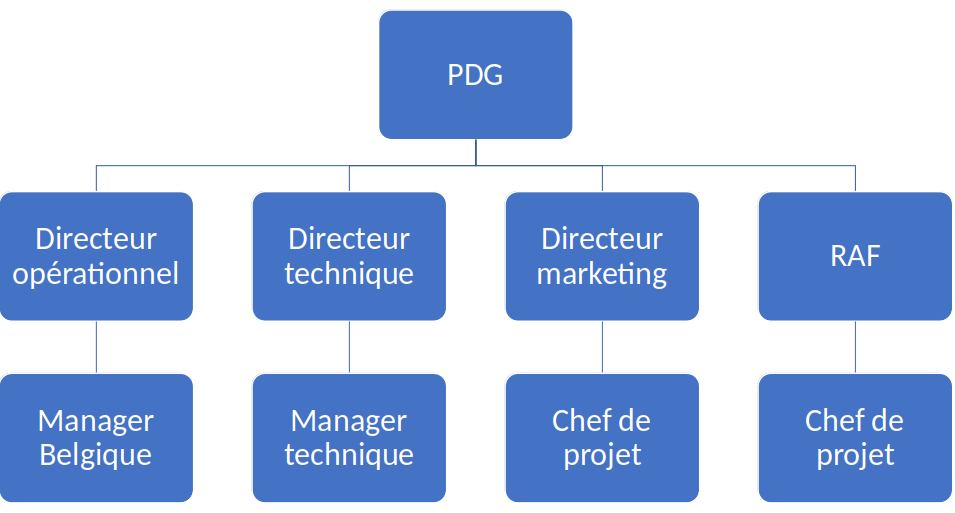
\includegraphics[scale=0.8,width=400px]{./Template LaTeX/Images/og.png}
	\centering
	\caption{Organigramme du CADORIM}
\end{figure}
\begin{comment}
	content...

\subsection{Planification du projet}
J'effectuais le diagramme de Gantt, pour avoir une meilleure compréhension de la chronologie des étapes de mon projet.
\newline
\newline
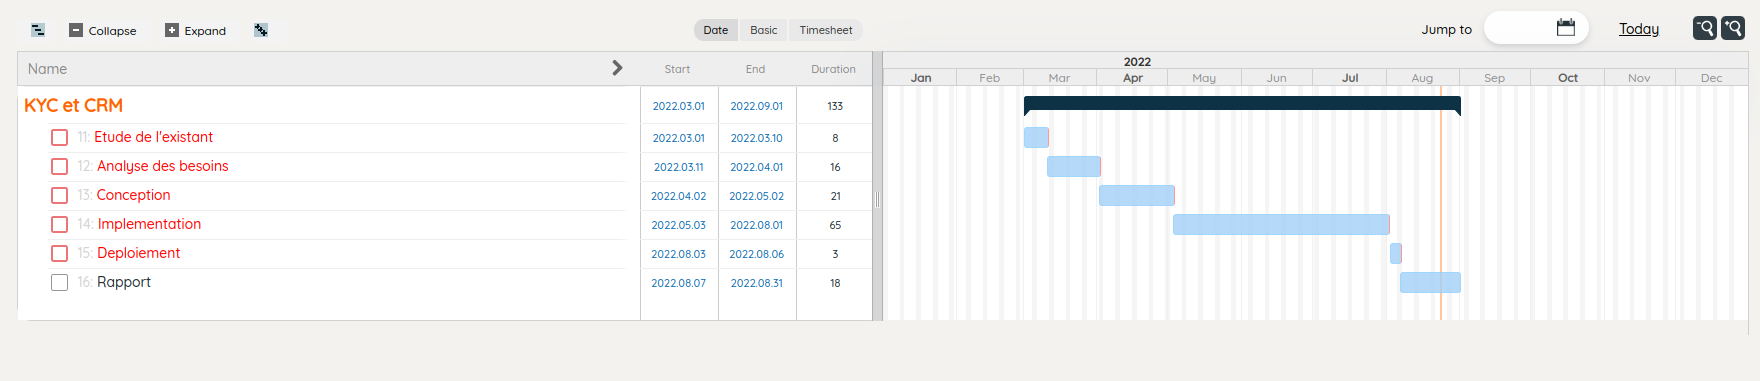
\includegraphics[width=500px,height=175px]{./Template LaTeX/Images/gantt.png}
\newline
Le projet est subdivisé en plusieurs phases.
\begin{enumerate}
\item Une phase comprenant l’étude de l’existant et analyse des besoins, en
intervenant les différents acteurs du projet.
\item Une phase de conception consistant à modéliser et formaliser les
données brutes du cahier de charge
\item Une phase d’implémentation consiste à traduire techniquement les
données provenant de la conception.
\item Déploiement : externalisation des ressources.
\end{enumerate}
\end{comment}
\newpage
\section{Description du projet}
%%%%%%%%%%%%%%%%%%%%%%%%%%%%%%%%%%%%% New add from Introduction %%%%%%%%%%%%%%%%%%%%%
\begin{comment}
	content...

Savoir qui est votre client et adopter des protocoles pour prévenir la criminalité financière sont des défis permanents pour les institutions financières. De manière significative, les institutions financières (y compris les banques, les coopératives de crédit et les sociétés financières du Fortune 50) doivent se conformer à un ensemble des réglementations de plus en plus complexes pour la vérification de l'identité des clients appelée KYC.

KYC, également connu sous le nom de "Know Your Customer" ou "Know Your Client", est un ensemble de procédures permettant de vérifier l'identité d'un client avant ou pendant les transactions avec les banques et autres institutions financières. Le respect des réglementations KYC peut aider à tenir à distance le blanchiment d'argent, le financement du terrorisme et d'autres stratagèmes de fraude courants. En vérifiant d'abord l'identité et les intentions d'un client au moment de l'ouverture du compte, puis en comprenant ses habitudes de transaction, les institutions financières sont en mesure d'identifier plus précisément les activités suspectes. 

Les institutions financières sont soumises à des normes de plus en plus strictes en matière de lois KYC. Ils doivent dépenser plus d'argent pour se conformer à KYC ou être passibles de lourdes amendes. Ces réglementations signifient que presque toutes les entreprises, plateformes ou organisations qui interagissent avec une institution financière pour ouvrir un compte ou effectuer des transactions devront se conformer à ces obligations.

La gestion de la relation client (CRM) est la combinaison de pratiques, de stratégies et de technologies que les entreprises utilisent pour gérer et analyser les interactions et les données client tout au long du cycle de vie du client. L'objectif est d'améliorer les relations de service client, de contribuer à la fidélisation de la clientèle et de stimuler la croissance des ventes. Les systèmes CRM compilent les données client à travers différents canaux, ou points de contact, entre le client et l'entreprise, qui peuvent inclure le site Web de l'entreprise, le téléphone, le chat en direct, le publipostage, les supports marketing et les réseaux sociaux. Les systèmes CRM peuvent également donner aux membres du personnel en contact avec les clients des informations détaillées sur les informations personnelles des clients, l'historique des achats, les préférences et les préoccupations d'achat.


\subsection{Motivations}    

KYC est un moyen de rendre la vérification de l'identité des clients plus précise et moins vulnérable à la fraude.

KYC doivent être effectuées lors de l'intégration d'un nouveau client, mais il est préférable de répéter ces vérifications de temps en temps, pour s'assurer que tout est comme il se doit. En surveillant les comptes clients de cette manière, les comportements suspects peuvent être signalés plus rapidement.

Un système CRM fournit des flux de travail automatisés qui permettent à votre équipe marketing de consacrer plus de temps à des tâches stratégiques, telles que la création de campagnes marketing qui résonnent, l'analyse des données de ces campagnes et le test de différentes approches basées sur ces analyses. Les agents du service client peuvent passer leur temps à travailler avec des clients qui ont des questions, des problèmes ou des besoins plus complexes. En bref, avec des processus de service client plus efficaces, les entreprises peuvent établir de meilleures relations avec leurs clients.
\end{comment}
\subsection{Problématiques}	

En réalité, la réalisation d'une application,qui applique le principe de KYC et integre un  système CRM,
nécessite
de faire face à des problématiques diverses et complexes. Ainsi, la société a décidé de se contenter,
dans un premier temps, Mise en place d’un système d’extration des donnees à partir des images (carte d'identité ou passeport) et traitement des ces donnees.
Ce sujet soulève de nombreuses questions aux implications différentes. Comment peut extraire le texte apartir de l'image? Comment sera-t-il traité ? Comment peut-il être utilisé dans le principe KYC ? Comment pouvons-nous obtenir un système CRM intégré ?


\subsection{Objectifs}

La mise en place d'une application pour appliquer l'ide de KYC en basant sur les différent technologie disponible . En basan sur l'extraction du text apartir d'une imange OCR on peut extracter la code MRZ apartir d'une imange du piece d'idendite ou passport est passe le code a un algorithem qui permer de d'etecter les information personnel.





	%\chapter{Conception du projet}
%\label{sec:EnvironnementDeTravail}
\chapter{Analyse fonctionnelle et conceptuelle}
\label{sec:Analyse fonctionnelle et conceptuelle}
%Durant la réalisation de ce projet, nous avons essayé d’utiliser différents
%outils de développement, d’une part afin de rendre la tâche de la
%réalisation plus facile, d’autre part pour que notre système soit robuste et
%répond parfaitement a nos besoins , et que nos interfaces soient claires et
%faciles à utiliser.

%\section{Choix de langage de modélisation :}
\section{Analyse fonctionnelle}
%Dans cette section, je présente le langage et le logiciel de modélisation que j’ai utilisé pour concevoir notre solution.
\begin{comment}
	content...

\subsection{UML}
On a utilisé UML comme langage de modélisation.
Langage de modélisation unifié UML (Unified modeling Langage) un
consiste a modéliser une application logicielle d'une façon standard
dans le cadre de conception orientée objet.
UML consiste a couvrir le cycle de vie d'un logiciel depuis la
spécification des besoins jusqu'au codage en offrant plusieurs
moyens de description et de modélisation des acteurs.
\section{Choix de logiciel de modélisation :}
\subsection{Visual Paradigm  en ligne} 
Visual Paradigm  en ligne est un outil de création de diagrammes en ligne. Vous pouvez créer un nombre illimité de diagrammes, graphiques et autres visuels à partir d’un large éventail de types de diagrammes, y compris UML, organigrammes, BPMN, ERD, DFD, ArchiMate et autres.
%%%%%%%%%%%%%%%%%%%%%%%%%%%%%%%%%%%%%%%%%%%%%%%%%%%%%%%%% Tests %%%%%%%%%%%%%%%%%%%%%%%%%%
\section{Diagramme UML}
\begin{comment}
\begin{table}
		
	\caption{Rôles des diagrammes UML utilisés.}
	\label{table:kysymys}
\begin{tabular}{|c|p{11cm}|}
	
	\hline
	\large \bfseries Diagramme & \large \bfseries Rôle\\
	\hline
	Diagramme de cas d’utilisation & Il consiste à donner une vision globale sur les principales fonctionnalités
	(chaque fonctionnalité représente un cas d’utilisateur) d’une application .  \\
	\hline
	Diagramme d’activité &  Fournir une vue du comportement d'un système en décrivant la séquence d'actions d'un processus.    \\
	\hline
	Diagramme de séquence &Permettent d'identifier les classes requises par un système et le comportement des objets de classes au cours des interactions.  \\
	\hline
	Diagramme de classe    &Le diagramme de classes représente généralement un schéma utilisé en génie
	logiciel pour modéliser un problème bien précis, sous forme des classes et des
	interfaces ainsi que les différentes relations entre celles-ci. \\
	\hline
	
\end{tabular}

\end{table}
\end{comment}
%Table \ref{table:kysymys} on page \pageref{table:kysymys} refers to the ...

\subsection{Diagramme de cas d’utilisation}
\begin{figure}[h!]
	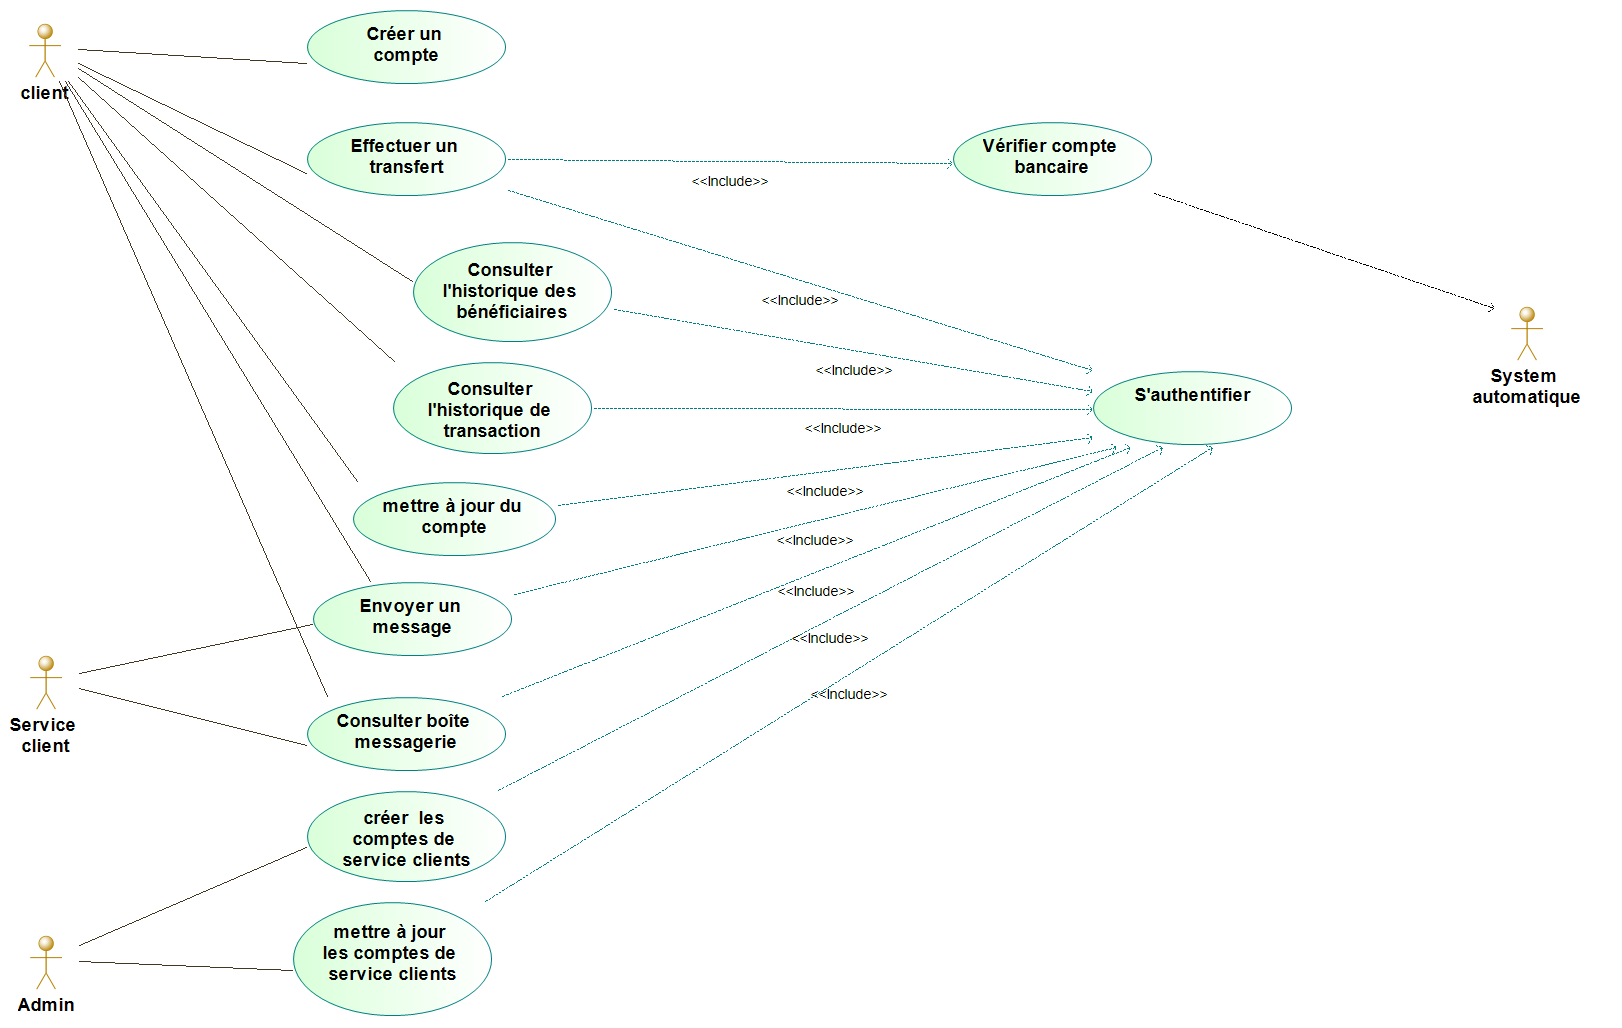
\includegraphics[width=18cm, height=12cm]{./Template LaTeX/Images/use_case.png}
	\caption{Diagramme de cas d’utilisation.}
	\label{fig1:use_case}
\end{figure}
%\textbf{Description détaillée des cas d'utilisation :}
\begin{comment}

\begin{table}[h]
	\begin{tabular}{|m{5cm}|m{2cm}|m{10cm}|}
		\hline
		\textbf{Cas d’utilisation} & \textbf{Acteur} & \textbf{Description}\\
		\hline
		\textbf{Créer un compte }&Client&L'utilisateur se renseigne pour créer un compte au sein de Cadorim pour
		pouvoir accéder au fonctionnalités proposées .\\
		\hline
		\textbf{S’authentifier}&Client&L'utilisateur saisit son identifiant et son mot de passe pour
		accéder aux fonctionnalités.\\
		\hline
		\textbf{Effectuer un transfert}&Client&L'utilisateur saisi le numéro du bénéficiaire et le montant a transférer.
		Une page de vérification avec les informations saisies.
		Transfère le montant vers le bénéficiaire.\\
		\hline
		\textbf{Créer un compte}&Client&L'utilisateur se renseigne pour créer un compte au sein de mauripay pour
		pouvoir accéder au fonctionnalités proposées .\\
		\hline
		\textbf{Créer un compte}&Client&L'utilisateur se renseigne pour créer un compte au sein de mauripay pour
		pouvoir accéder au fonctionnalités proposées .\\
		\hline
		\textbf{Créer un compte}&Client&L'utilisateur se renseigne pour créer un compte au sein de mauripay pour
		pouvoir accéder au fonctionnalités proposées .\\
		\hline
		
	
			
	\end{tabular}
	\caption{Description détaillée des cas d'utilisation}
	\label{4.1}
\end{table}
\end{comment}


	%\textbf{• Description détaillée des cas d'utilisation  :}
\begin{comment}
	
\begin{table}[h]
	\begin{tabular}{|m{4cm}|m{13.5cm}|}
		\hline
		\textbf{Cas d’utilisation}   \textbf{Description}\\
		\hline
		Créer un compte&L'utilisateur se renseigne pour créer un compte au sein de Cadorim pour
		pouvoir accéder au fonctionnalités proposées .\\
		\hline
		S’authentifier&L'utilisateur saisit son identifiant et son mot de passe pour
		accéder aux fonctionnalités.\\
		\hline
		Effectuer un transfert&L'utilisateur saisi le montant a transférer et les informations de  bénéficiaire.
		\newline Une page de vérification avec les informations saisies.
		\newline Transfère le montant vers le bénéficiaire.\\
		\hline
		Consulter l'historique des bénéficaires&L'utilisateur peut voire liste des bénéficaires \\
		\hline
		Consulter l'historique des transactions&L'utilisateur peut voire liste des transactions\\
		\hline
		mettre à jour du compte&L'utilisateur se renseigne pour créer un compte au sein de mauripay pour
		pouvoir accéder au fonctionnalités proposées .\\
		\hline
		Envoyer un message&L'utilisateur se renseigne pour créer un compte au sein de mauripay pour
		pouvoir accéder au fonctionnalités proposées .\\
		\hline
			Consulter boite \newline messagerie&L'utilisateur se renseigne pour créer un compte au sein de mauripay pour
		pouvoir accéder au fonctionnalités proposées .\\
		\hline
		
		
		
	\end{tabular}
	\caption{Description détaillée des cas d'utilisation d'acteur client}
	\label{4.1}
\end{table}
	content...
\end{comment}
%\newpage
\textbf{\hspace*{-1cm}• Description détaillée des cas d'utilisation  :\newline}
\begin{table}[h]
	\hspace*{-2cm}
	\begin{tabular}{|m{19.8cm}|}
		\hline
		\begin{center}
		 \textbf{Cas d’utilisation : Créer un compte, S’authentifier et Créer les comptes de service clients }
		\end{center}
		\\
		[-4ex] 
		\hline
			\begin{tabular}{m{3cm}|m{14cm}}
			
				\centering 	\textbf{Titre} & Créer un compte , S’authentifier , Créer les comptes de service clients
				\\
				[0ex] 
			\end{tabular}
		\\
		
		\hline
			\begin{tabular}{m{3cm}|m{14cm}}
			
			\centering 	\textbf{But} & Créer un compte pour accéder aux fonctionnalités de l’application 	\\
			[0ex] 
			
		\end{tabular}
		\\
		\hline
			\begin{tabular}{m{3cm}|m{15.5cm}}
			
			\centering 	\textbf{Résumé} & L'utilisateur doit remplir un formulaire d’inscription et identifier électroniquement leur document comme des pièces d’identité (carte d’identité, passeport ) à partir de leur caméra du téléphone puis valide son action.\newline Le système effectue une vérification puis une mise à jour de la base de données.
			\\
			[0ex] 
		\end{tabular}
		\\
		
		\hline
			\begin{tabular}{m{3cm}|m{14cm}}
			
			\centering 	\textbf{Acteurs } & Client,Admin \\[0ex]
			
		\end{tabular}
		\\
		 
		\hline
		\begin{center}
			\textbf{Descriptions des enchainements}
		\end{center}
		\\
		[-4ex] 
		\hline	
			\begin{tabular}{m{9.3cm}|m{9.3cm}}
			
			\begin{center}
				\textbf{Pré condition}
			\end{center}
		 		& 
		 	\begin{center}
				\textbf{Post condition}
			\end{center}
			\\[-4ex]
		\end{tabular}
		\\
		
		\hline
			\begin{tabular}{m{9.3cm}|m{9.3cm}}
			L'utilisateur doit accéder au système
			& 
			L'utilisateur inscrit
		\end{tabular}
		\\
		\hline
			\begin{center}
			\textbf{Scenario nominal}
			\end{center}
		\\
		[-4ex]
		\hline
		\begin{enumerate}
			\item [1.] L’utilisateur demande la page d’inscription en cliquant sur «S'INSCRIRE»
			\item [2.] Le système lui envoie la page d’inscription
			\item [3.] L’utilisateur rempli le formulaire et scanne leur document puis appuie sur S'INSCRIRE
			\item [4.] Le système effectue les validations et l’enregistrement dans la base de données
			\item [5.] L’utilisateur est redirigé vers la page d’authentification et renseigne ses identifiants en cas d'acteur client 
		\end{enumerate}
		\\
		[-4ex]
		\hline	
			\begin{center}
			\textbf{Enchainement d’échec }
		\end{center}
		\\ 
		[-4ex]
		\hline
		\begin{tabular}{m{17.5cm}}
			\begin{enumerate}
				\item [6.] Le compte existe déjà ou les données saisies sont incorrectes
				\item [7.] Il n’y a pas de connexion internet
			\end{enumerate}
			\\[-4ex]
		\end{tabular}
		\\
		\hline	
		
	\end{tabular}
	\centering \caption{Description détaillée des cas d'utilisation : Créer un compte  et S’authentifier}
	\label{4.1}
\end{table}
\newpage

\begin{table}[h]
	\hspace*{-2cm}
	\vspace*{-2cm}
	\begin{tabular}{|m{19.8cm}|}
		\hline
		\begin{center}
			\textbf{Cas d’utilisation : Effectuer transfert}
		\end{center}
		\\
		[-4ex] 
		\hline
		\begin{tabular}{m{3cm}|m{14cm}}
			
			\centering 	\textbf{Titre} & Effectuer transfert
			\\
			[0ex] 
		\end{tabular}
		\\
		
		\hline
		\begin{tabular}{m{3cm}|m{14cm}}
			
			\centering 	\textbf{But} & Envoyer de l’argent à un bénéficiaire	\\
			[0ex] 
			
		\end{tabular}
		\\
		\hline
		\begin{tabular}{m{3cm}|m{15.5cm}}
			
			\centering 	\textbf{Résumé} & L’utilisateur saisit les informations du bénéficiaire et le montant de la transaction et valide. Le système envoyait les informations de la carte bancaire au  fournisseur de paiement  avant de finaliser l’opération.
			\\
			[0ex] 
		\end{tabular}
		\\
		
		\hline
		\begin{tabular}{m{3cm}|m{14cm}}
			
			\centering 	\textbf{Acteurs } & Client \\[0ex]
			
		\end{tabular}
		\\
		
		\hline
		\begin{center}
			\textbf{Descriptions des enchainements}
		\end{center}
		\\
		[-4ex] 
		\hline	
		\begin{tabular}{m{9.3cm}|m{9.3cm}}
			
			\begin{center}
				\textbf{Pré condition}
			\end{center}
			& 
			\begin{center}
				\textbf{Post condition}
			\end{center}
			\\[-4ex]
		\end{tabular}
		\\
		
		\hline
		\begin{tabular}{m{9.3cm}|m{9.3cm}}
			- L’utilisateur doit se connecter \newline
			- L’utilisateur doit utiliser une carte bancaire valide & 
			- Le transfert est effectué \newline
			- Afficher  l'historique des transactions
			\\[0ex]
		\end{tabular}
		\\
		\hline
		\begin{center}
			\textbf{Scenario nominal}
		\end{center}
		\\
		[-4ex]
		\hline
		\begin{enumerate}
			\item [1.] L’utilisateur accède au formulaire de transfert en saisit le montant puis  cliquant sur « Envoyer »
			\item [2.] Le système lui demande de saisir les informations de transfert
			\item [3.] L’utilisateur rempli le formulaire appuie sur le bouton « Valider »
			\item [4.] Le système débiter le compte de cadorim et crédité le compte de bénéficiaire
			\item [5.] Le système lui affiche la page de l'historique des transactions
		\end{enumerate}
		\\
		[-4ex]
		\hline	
		\begin{center}
			\textbf{Enchainement d’échec }
		\end{center}
		\\ 
		[-4ex]
		\hline
		\begin{tabular}{m{17.5cm}}
			\begin{enumerate}
				\item [6.] La carte bancaire invalide ou le solde est insuffisant
				\item [7.] La saisie de données n’est pas correcte
				\item [8.] La connexion n’est pas bonne pour effectuer et suivre un transfert
			\end{enumerate}
			\\[-4ex]
		\end{tabular}
		\\
		\hline	
		
	\end{tabular}
	\vspace*{1.5cm}
	\centering \caption{Description détaillée des cas d'utilisation : Effectuer transfert}
	\label{4.1}
\end{table}

\newpage

\begin{table}[h]
	\hspace*{-2cm}
	\vspace*{-2.5cm}
	\begin{tabular}{|m{19.8cm}|}
		\hline
		\begin{center}
			\textbf{Cas d’utilisation : Consulter l'historique des bénéficiaires et l'historique de transaction}
		\end{center}
		\\
		[-4ex] 
		\hline
		\begin{tabular}{m{3cm}|m{14cm}}
			
			\centering 	\textbf{Titre} & Consulter l'historique des bénéficiaires,Consulter l'historique de transaction
			\\
			[0ex] 
		\end{tabular}
		\\
		
		\hline
		\begin{tabular}{m{3cm}|m{14cm}}
			
			\centering 	\textbf{But} & Consultations de l'historique\\
			[0ex] 
			
		\end{tabular}
		\\
		\hline
		\begin{tabular}{m{3cm}|m{15.5cm}}
			
			\centering 	\textbf{Résumé} & L'utilisateur voit les renseignements sur le bénéficiaire et l'opération de transaction.
			\\
			[0ex] 
		\end{tabular}
		\\
		
		\hline
		\begin{tabular}{m{3cm}|m{14cm}}
			
			\centering 	\textbf{Acteurs } & Client \\[0ex]
			
		\end{tabular}
		\\
		
		\hline
		\begin{center}
			\textbf{Descriptions des enchainements}
		\end{center}
		\\
		[-4ex] 
		\hline	
		\begin{tabular}{m{9.3cm}|m{9.3cm}}
			
			\begin{center}
				\textbf{Pré condition}
			\end{center}
			& 
			\begin{center}
				\textbf{Post condition}
			\end{center}
			\\[-4ex]
		\end{tabular}
		\\
		
		\hline
		\begin{tabular}{m{9.3cm}|m{9.3cm}}
			- L’utilisateur doit se connecter \newline
			 & 
			- Afficher  l'historique des transactions ou des  \newline bénéficiaires
			\\[0ex]
		\end{tabular}
		\\
		\hline
		\begin{center}
			\textbf{Scenario nominal}
		\end{center}
		\\
		[-4ex]
		\hline
		\begin{enumerate}
			\item [1.] L’utilisateur accède a l'historique des transactions ou des bénéficiaires en cliquant sur « Transferts » ou « Benef »
			\item [2.] Le système lui affiche la page de l'historique
		\end{enumerate}
		\\
		[-4ex]
		\hline	
		\begin{center}
			\textbf{Enchainement d’échec }
		\end{center}
		\\ 
		[-4ex]
		\hline
		\begin{tabular}{m{17.5cm}}
			\begin{enumerate}
				\item [3.] Il n’y a pas de connexion internet
				
			\end{enumerate}
			\\[-4ex]
		\end{tabular}
		\\
		\hline	
		
	\end{tabular}
	\vspace*{2cm}
	\centering \caption{Description détaillée des cas d'utilisation : Consulter l'historiques(des transactions ou des bénéficiaires)}
	\label{4.1}
\end{table}

\newpage

\begin{table}[h]
	\hspace*{-2cm}
	\vspace*{-2cm}
	\begin{tabular}{|m{19.8cm}|}
		\hline
		\begin{center}
			\textbf{Cas d’utilisation : Consulter boite messagerie}
		\end{center}
		\\
		[-4ex] 
		\hline
		\begin{tabular}{m{3cm}|m{14cm}}
			
			\centering 	\textbf{Titre} & Consulter boite messagerie
			\\
			[0ex] 
		\end{tabular}
		\\
		
		\hline
		\begin{tabular}{m{3cm}|m{14cm}}
			
			\centering 	\textbf{But} & Consulter boite messagerie\\
			[0ex] 
			
		\end{tabular}
		\\
		\hline
		\begin{tabular}{m{3cm}|m{15.5cm}}
			
			\centering 	\textbf{Résumé} &L'utilisateur voit l'historique des  messages et les messages reçus.
			\\
			[0ex] 
		\end{tabular}
		\\
		
		\hline
		\begin{tabular}{m{3cm}|m{14cm}}
			
			\centering 	\textbf{Acteurs } & Client, Srvice client \\[0ex]
			
		\end{tabular}
		\\
		
		\hline
		\begin{center}
			\textbf{Descriptions des enchainements}
		\end{center}
		\\
		[-4ex] 
		\hline	
		\begin{tabular}{m{9.3cm}|m{9.3cm}}
			
			\begin{center}
				\textbf{Pré condition}
			\end{center}
			& 
			\begin{center}
				\textbf{Post condition}
			\end{center}
			\\[-4ex]
		\end{tabular}
		\\
		
		\hline
		\begin{tabular}{m{9.3cm}|m{9.3cm}}
			- L’utilisateur doit se connecter \newline
			& 
			- Afficher  l'historique des  messages et les messages reçus
			\\[0ex]
		\end{tabular}
		\\
		\hline
		\begin{center}
			\textbf{Scenario nominal}
		\end{center}
		\\
		[-4ex]
		\hline
		\begin{enumerate}
			\item [1.] L’utilisateur accède à la boîte messagerie
			\item [2.] Le système lui affiche la page des messageries
		\end{enumerate}
		\\
		[-4ex]
		\hline	
		\begin{center}
			\textbf{Enchainement d’échec }
		\end{center}
		\\ 
		[-4ex]
		\hline
		\begin{tabular}{m{17.5cm}}
			\begin{enumerate}
				\item [3.] Il n’y a pas de connexion internet
				
			\end{enumerate}
			\\[-4ex]
		\end{tabular}
		\\
		\hline	
		
	\end{tabular}
	\vspace*{1.5cm}
	\centering \caption{Description détaillée des cas d'utilisation : Consulter boite messagerie}
	\label{4.1}
\end{table}


\newpage

\begin{table}[h]
	\hspace*{-2cm}
	\vspace*{-2cm}
	\begin{tabular}{|m{19.8cm}|}
		\hline
		\begin{center}
			\textbf{Cas d’utilisation : Envoyer un message}
		\end{center}
		\\
		[-4ex] 
		\hline
		\begin{tabular}{m{3cm}|m{14cm}}
			
			\centering 	\textbf{Titre} & Envoyer un message
			\\
			[0ex] 
		\end{tabular}
		\\
		
		\hline
		\begin{tabular}{m{3cm}|m{14cm}}
			
			\centering 	\textbf{But} & Envoyer un message\\
			[0ex] 
			
		\end{tabular}
		\\
		\hline
		\begin{tabular}{m{3cm}|m{15.5cm}}
			
			\centering 	\textbf{Résumé} &L'utilisateur peut envoyer un message où répond à un message
			\\
			[0ex] 
		\end{tabular}
		\\
		
		\hline
		\begin{tabular}{m{3cm}|m{14cm}}
			
			\centering 	\textbf{Acteurs } & Client, Srvice client \\[0ex]
			
		\end{tabular}
		\\
		
		\hline
		\begin{center}
			\textbf{Descriptions des enchainements}
		\end{center}
		\\
		[-4ex] 
		\hline	
		\begin{tabular}{m{9.3cm}|m{9.3cm}}
			
			\begin{center}
				\textbf{Pré condition}
			\end{center}
			& 
			\begin{center}
				\textbf{Post condition}
			\end{center}
			\\[-4ex]
		\end{tabular}
		\\
		
		\hline
		\begin{tabular}{m{9.3cm}|m{9.3cm}}
			- L’utilisateur doit se connecter \newline
			& 
			\centering - Le message est envoyé
			\\[0ex]
		\end{tabular}
		\\
		\hline
		\begin{center}
			\textbf{Scenario nominal}
		\end{center}
		\\
		[-4ex]
		\hline
		\begin{enumerate}
			\item [1.] L’utilisateur demande le formulaire d’envoi de message
			\item [2.] Le système lui affiche la page des discussions
		\end{enumerate}
		\\
		[-4ex]
		\hline	
		\begin{center}
			\textbf{Enchainement d’échec }
		\end{center}
		\\ 
		[-4ex]
		\hline
		\begin{tabular}{m{17.5cm}}
			\begin{enumerate}
				\item [3.] Il n’y a pas de connexion internet
				
			\end{enumerate}
			\\[-4ex]
		\end{tabular}
		\\
		\hline	
		
	\end{tabular}
	\vspace*{1.5cm}
	\centering \caption{Description détaillée des cas d'utilisation : Envoyer un message}
	\label{4.1}
\end{table}
\begin{comment}

	\item[•]  \textbf{Description détaillée des cas d'utilisation d'acteur service client :}
\begin{table}[h]
	\begin{tabular}{|m{4cm}|m{13.5cm}|}
		\hline
		\textbf{Cas d’utilisation}  & \textbf{Description}\\
		\hline
		Enoyer un message&L'utilisateur se renseigne pour créer un compte au sein de Cadorim pour
		pouvoir accéder au fonctionnalités proposées .\\
		\hline
		S’authentifier&L'utilisateur saisit son identifiant et son mot de passe pour
		accéder aux fonctionnalités.\\
		\hline
			Consulter boite \newline messagerie&L'utilisateur saisit son identifiant et son mot de passe pour
		accéder aux fonctionnalités.\\
		\hline
	\end{tabular}
	\caption{Description détaillée des cas d'utilisation d'acteur service client}
	\label{4.1}
\end{table}

	\item[•]  \textbf{Description détaillée des cas d'utilisation d'acteur admin :}
\begin{table}[h]
	\begin{tabular}{|m{4cm}|m{13.5cm}|}
		\hline
		\textbf{Cas d’utilisation}  & \textbf{Description}\\
		\hline
		Créer les comptes de service clients&L'utilisateur se renseigne pour créer un compte au sein de Cadorim pour
		pouvoir accéder au fonctionnalités proposées .\\
		\hline
		S’authentifier&L'utilisateur saisit son identifiant et son mot de passe pour
		accéder aux fonctionnalités.\\
		\hline
		Mettre à jour les comptes de service clients&L'utilisateur saisit son identifiant et son mot de passe pour
		accéder aux fonctionnalités.\\
		\hline
	\end{tabular}
	\caption{Description détaillée des cas d'utilisation d'acteur admin}
	\label{4.1}
\end{table}
\item[•]  \textbf{Description détaillée des cas d'utilisation d'acteur system :}
\begin{table}[h]
	\begin{tabular}{|m{4cm}|m{13.5cm}|}
		\hline
		\textbf{Cas d’utilisation}  & \textbf{Description}\\
		\hline
		 Vérifier compte \newline bancaire&L'utilisateur se renseigne pour créer un compte au sein de Cadorim pour
		pouvoir accéder au fonctionnalités proposées .\\
		\hline
	\end{tabular}
	\caption{Description détaillée des cas d'utilisation d'acteur secondaire system}
	\label{4.1}
\end{table}
	content...
\end{comment}


\subsection{Diagramme d’activité}
Cette section a pour objectif de mettre en surbrillance le processus quelques fonctionnalités de
l’application pour voir les détailles. J’ai choisi trois cas d’utilisation, à savoir, la création d’un compte,la transfert d'argent et l'authentification.
\newpage
\subsubsection{Création de compte}
Le diagramme d’activité qu’illustre la figure~\ref{activiteCompte} décrit le cas d’utilisation « Créer un compte ».
\begin{figure}[h!]
	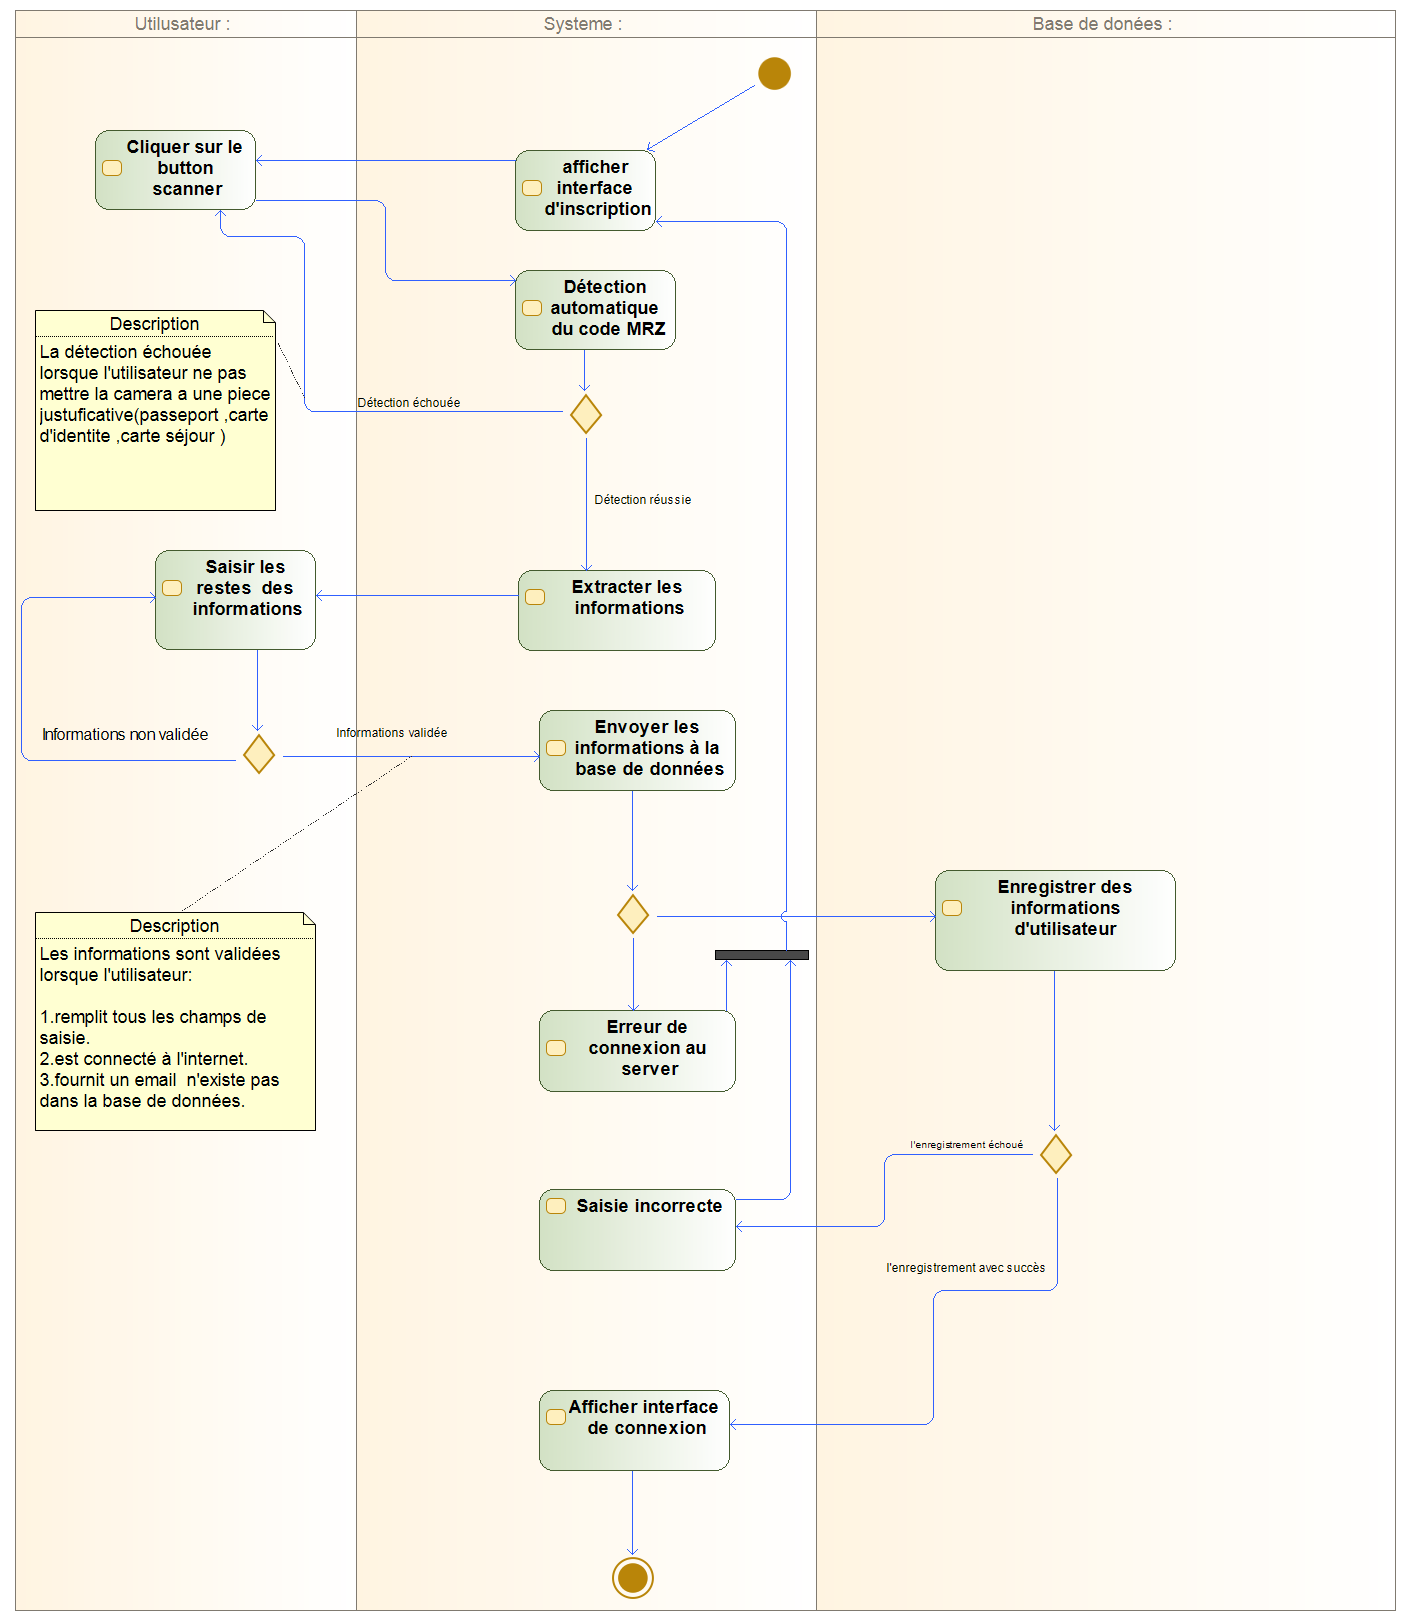
\includegraphics[width=18cm, height=19cm]{./Template LaTeX/Images/ins_act.png}
\caption{Diagramme d’activité : Création de compte}
\label{activiteCompte}

\end{figure}

\subsubsection{Transfert d'argent}
Le diagramme d’activité qu’illustre la figure~\ref{activiteTr} décrit les différentes actions ou enchainements
effectués lors d’une opération de transfert d’argent.
\begin{figure}[h!]
	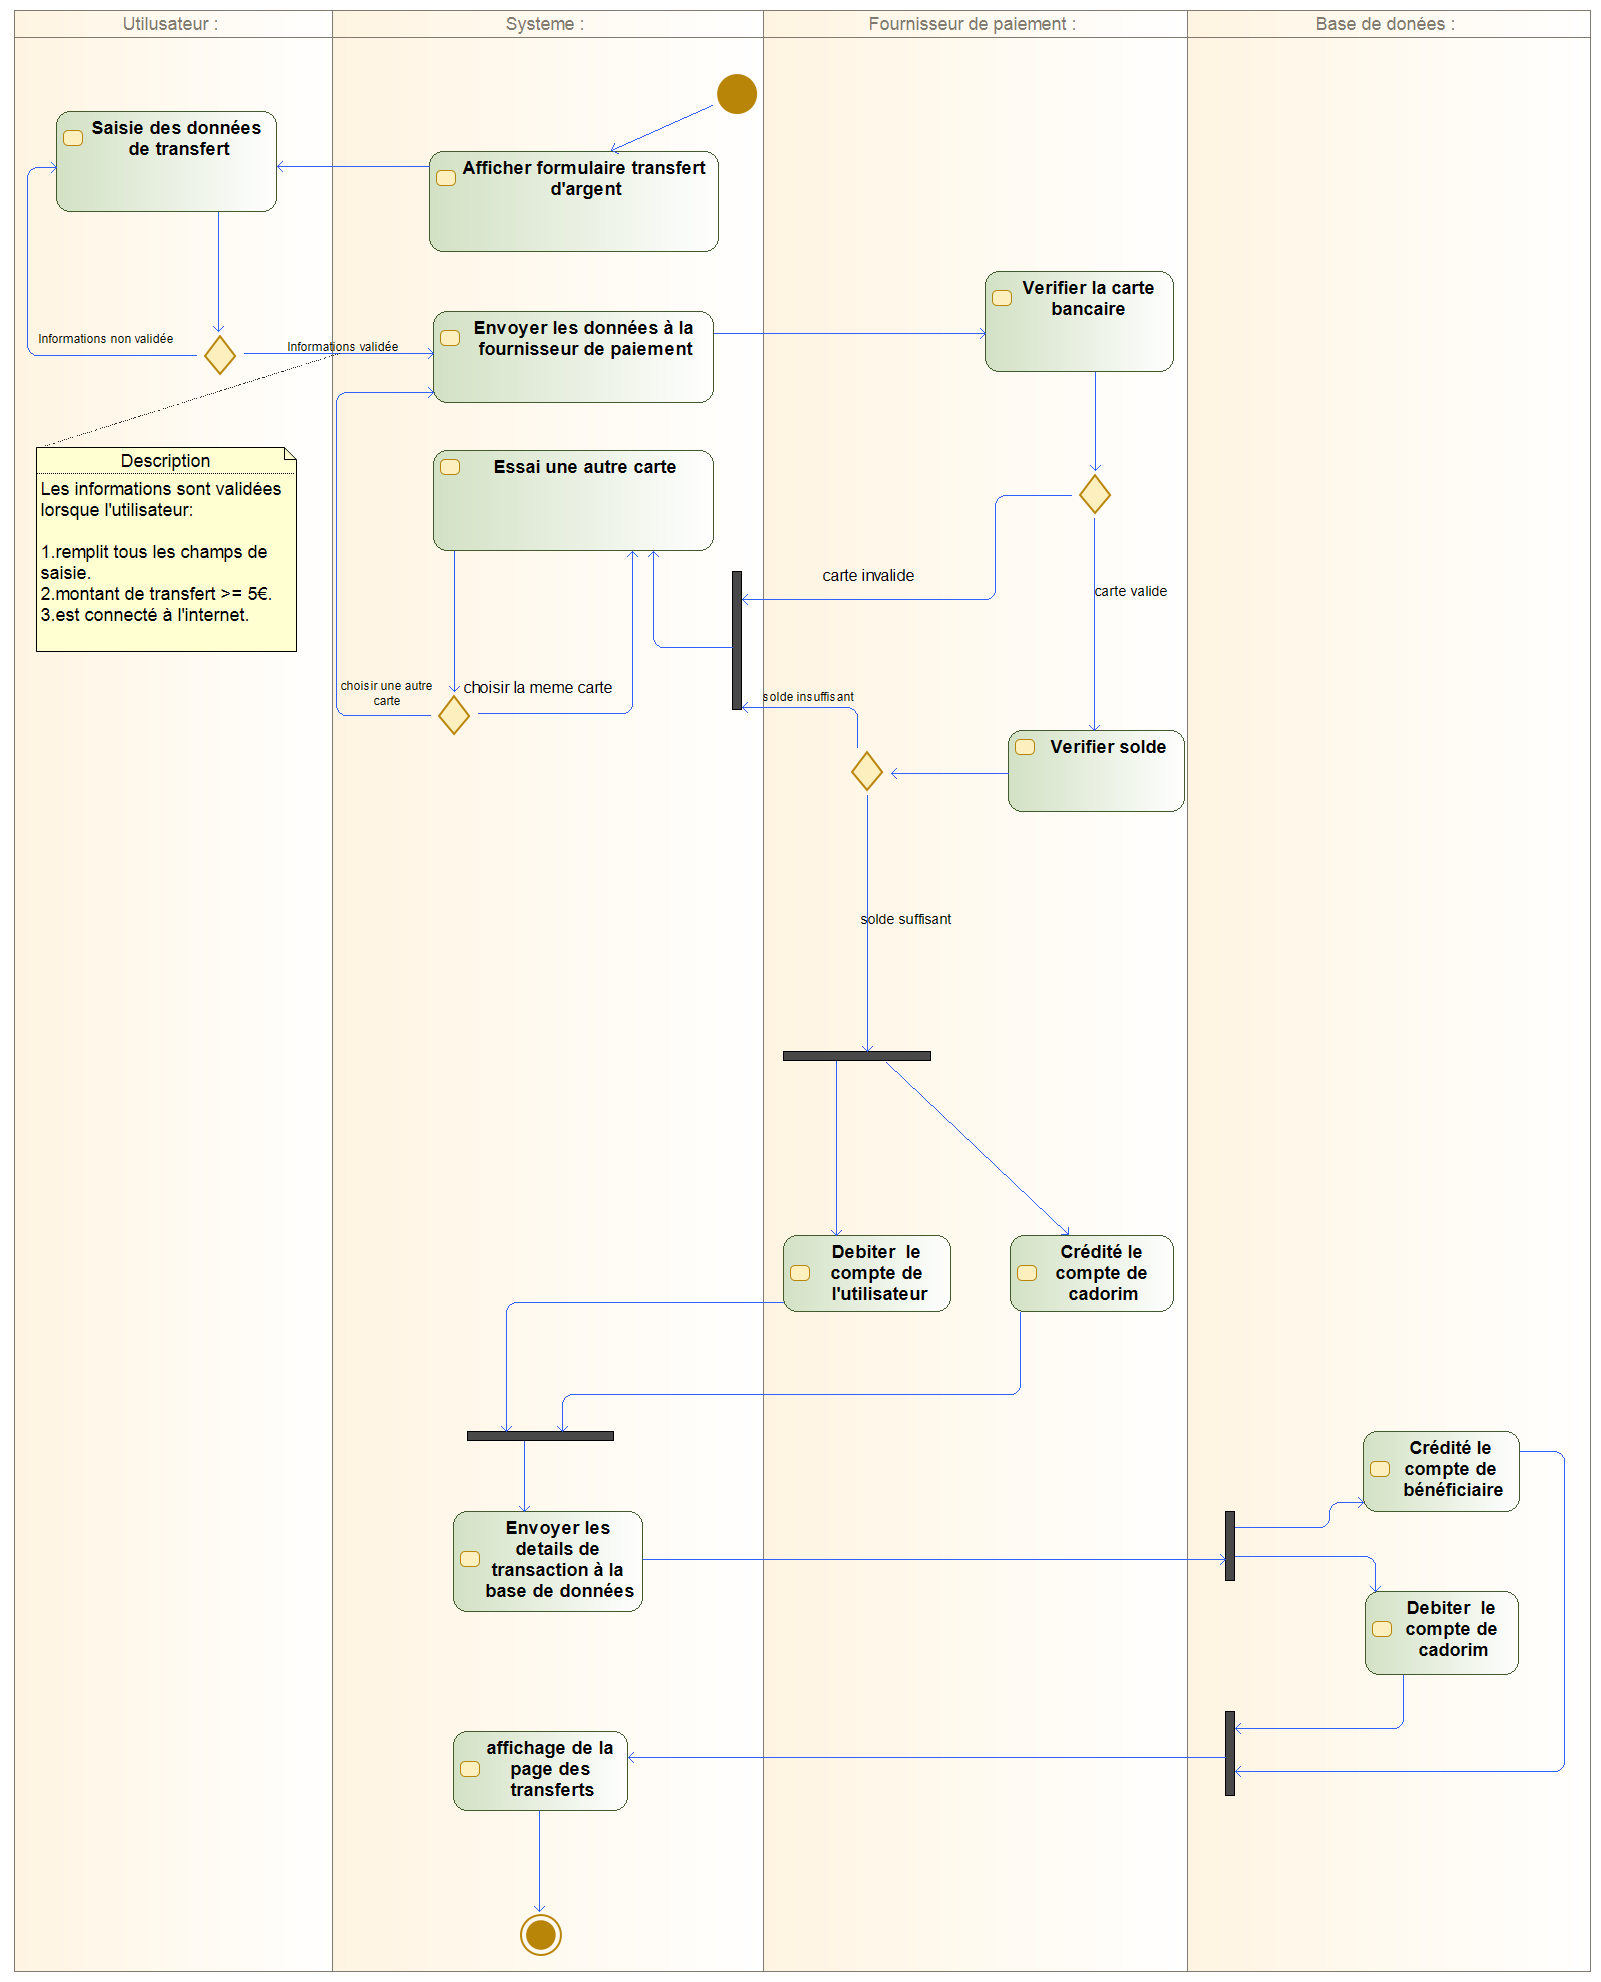
\includegraphics[width=18cm, height=20cm]{./Template LaTeX/Images/trans_act.png}
	\caption{Diagramme d'activité : Transfert d'argent}
	\label{activiteTr}
\end{figure}

\subsubsection{Authentification}
Le diagramme d’activité qu’illustre la figure~\ref{activiteAuth} décrit le cas d’utilisation « Authentification ».
\begin{figure}[h!]
	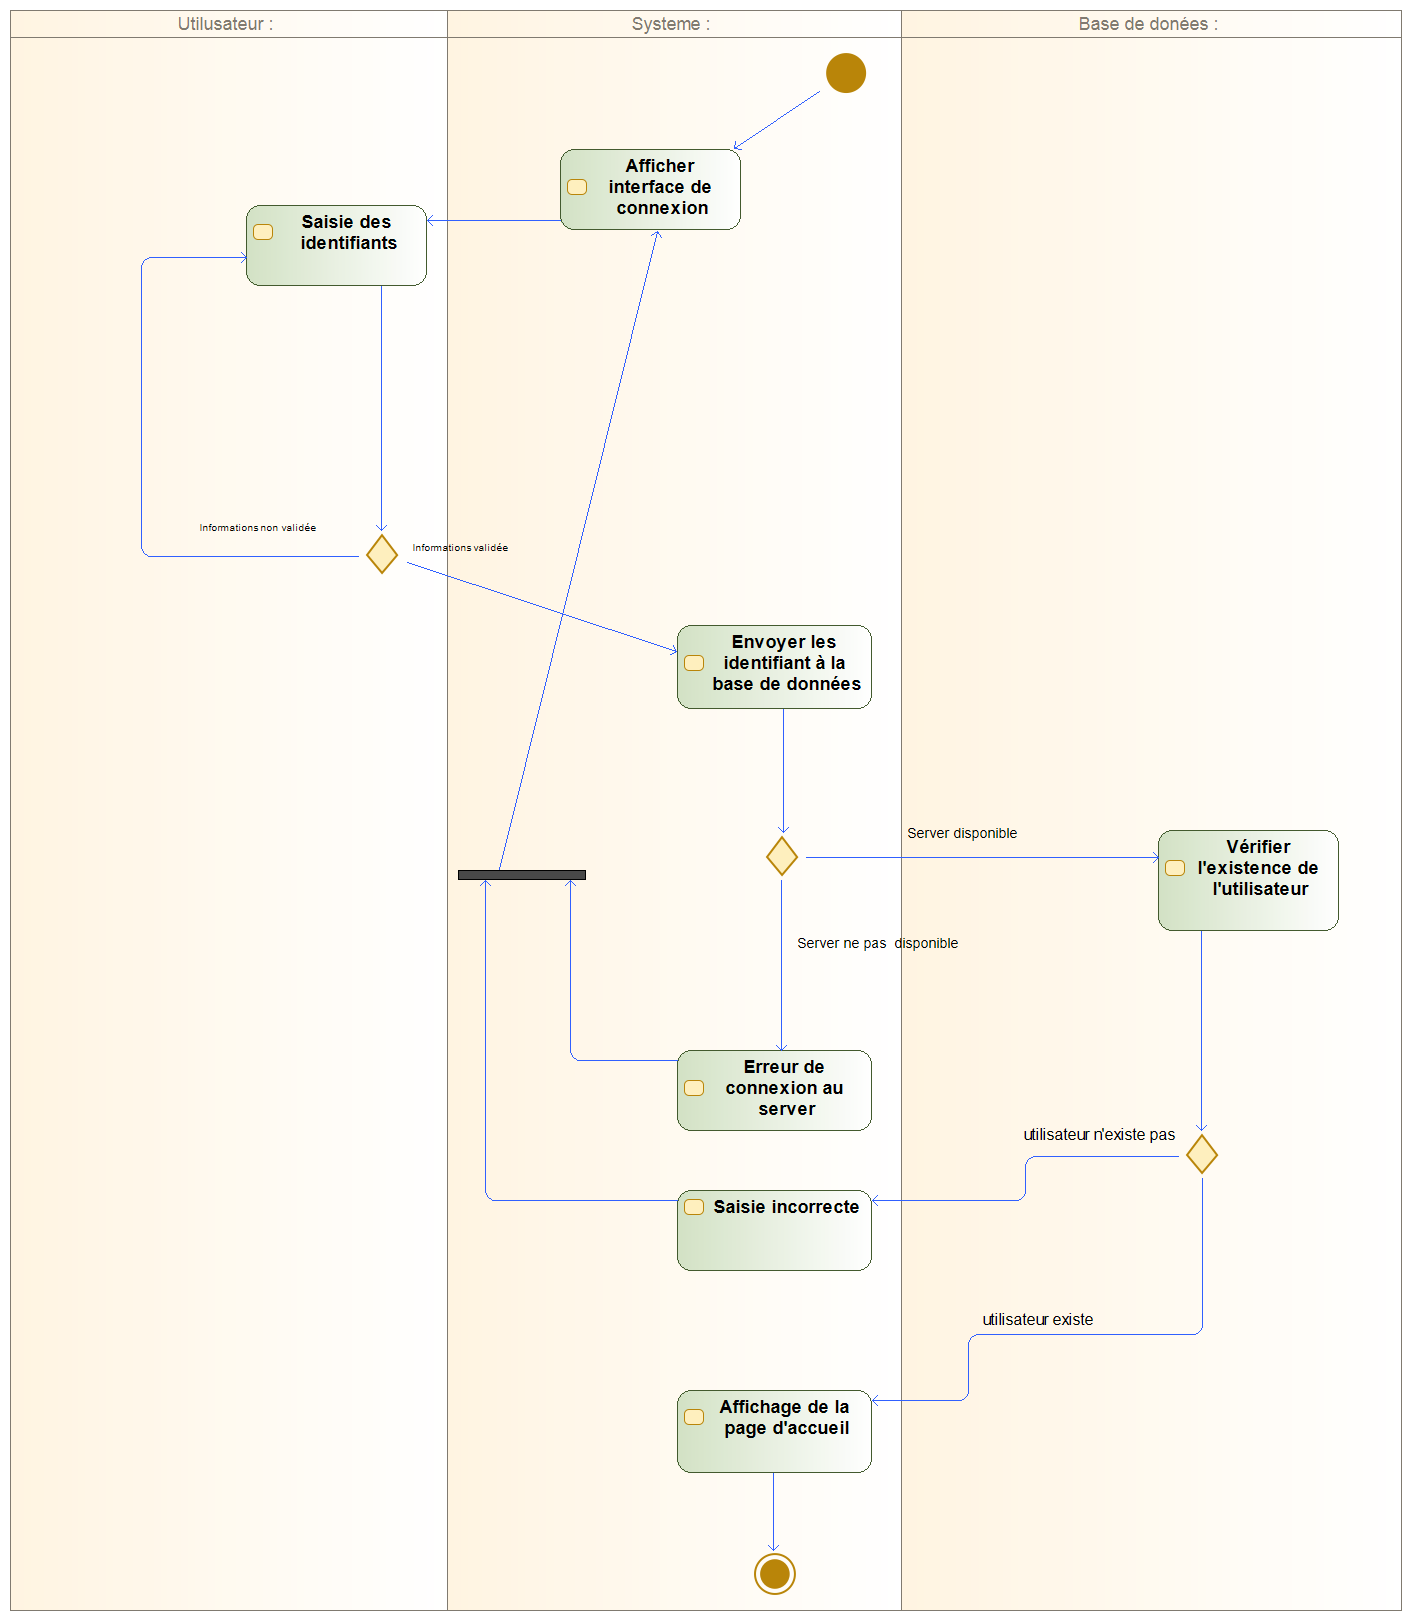
\includegraphics[width=18cm, height=20cm]{./Template LaTeX/Images/auth_act.png}
	\caption{Diagramme d'activité : Authentification}
	\label{activiteAuth}
\end{figure}


%\section{Modélisation de la base de données}
%\subsection{Diagramme de séquence}
%\newpage

\subsection{Diagramme de classe}
Afin de bien détailler l’architecture de la base de données, nous avons conçu le diagramme de
classe représenté dans la figure~\ref{fig4:class}.
\begin{figure}[h!]
	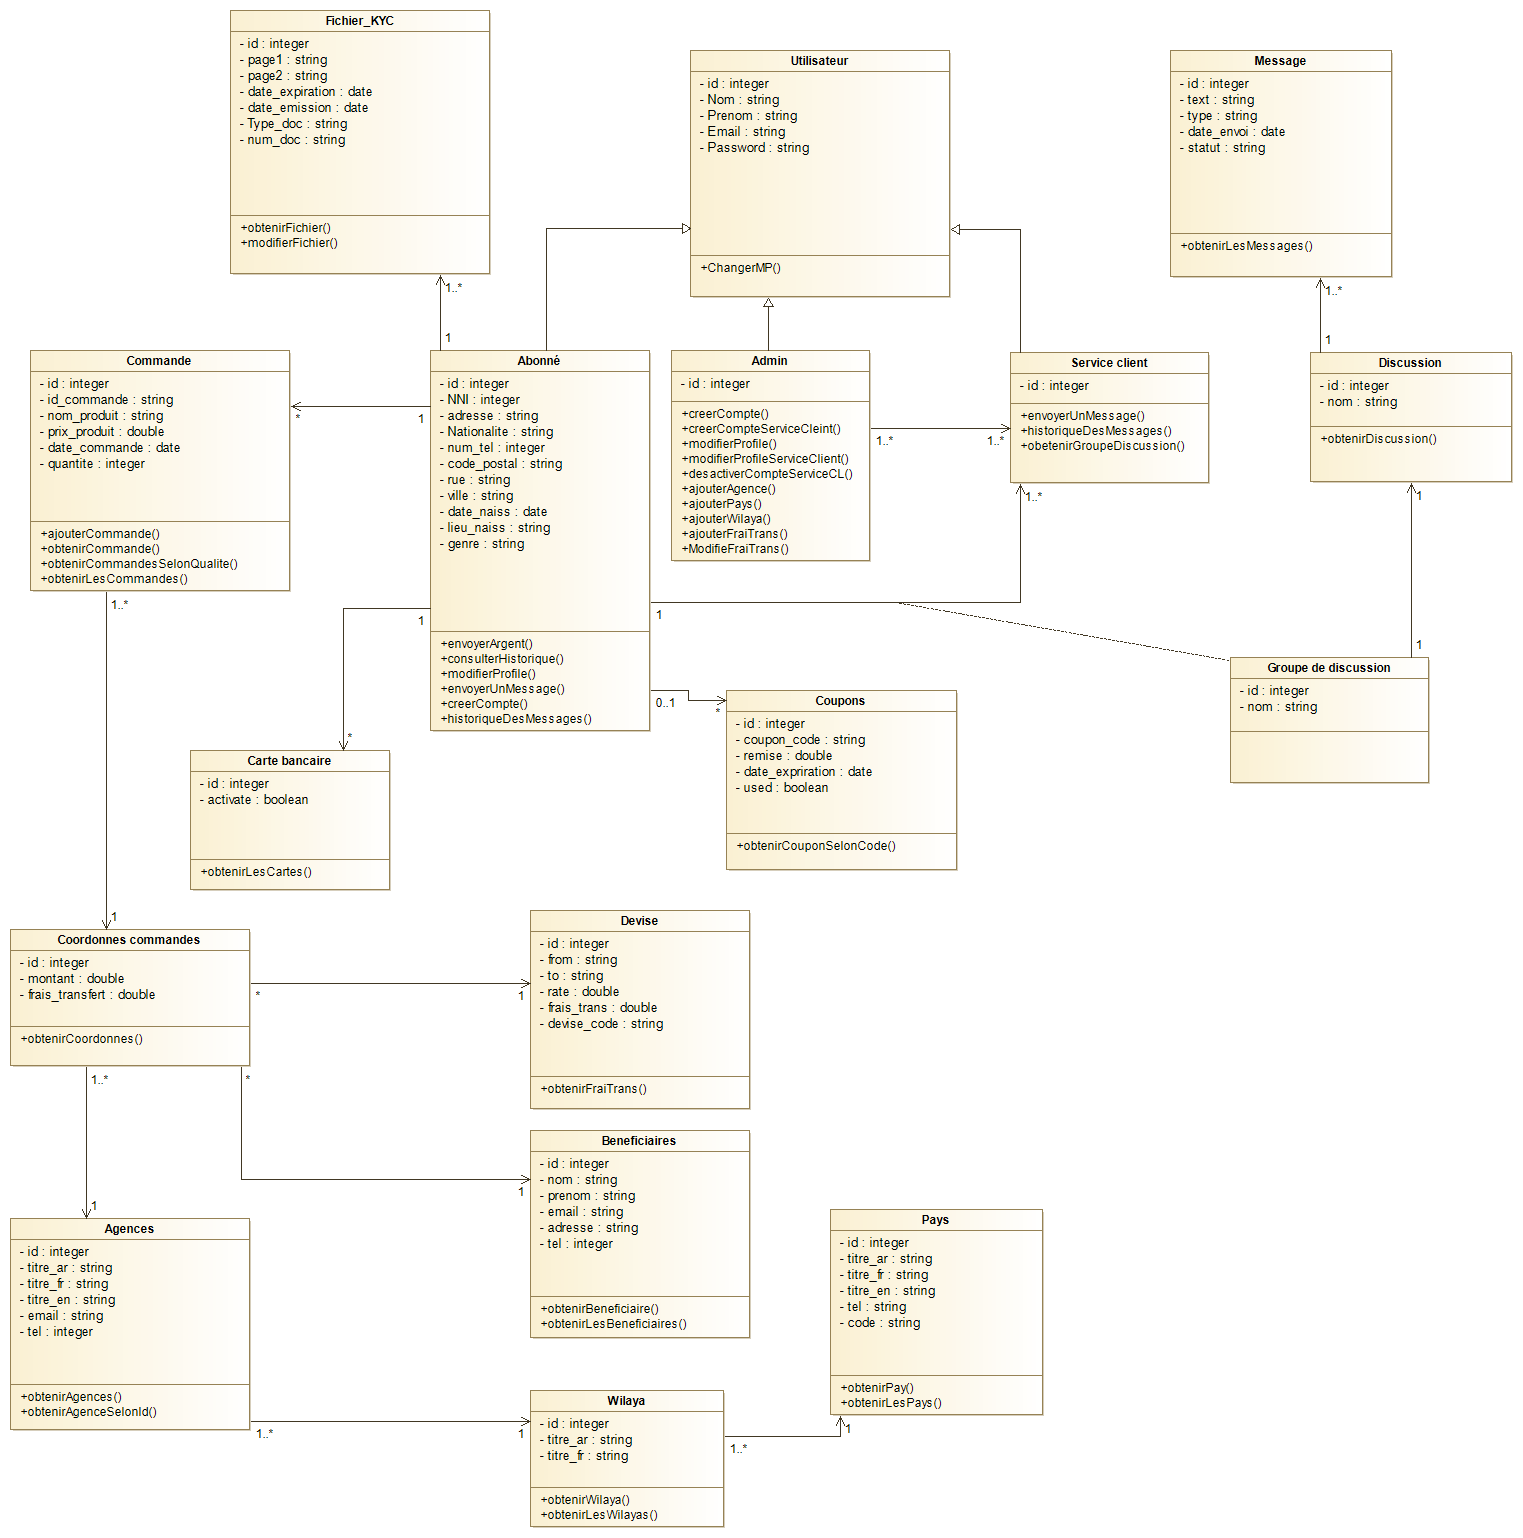
\includegraphics[width=18cm, height=20cm]{./Template LaTeX/Images/Diagramme_de_classe_V3.png}
	\caption{Diagramme de classe}
	\label{fig4:class}
\end{figure}
\newpage
\hspace*{-2cm} Le tableau~\ref{fig4:classT} explique les différentes classes de la base de données.
\begin{table}[h]
	\hspace*{-2cm}
	%\vspace*{6cm}
	\begin{tabular}{|m{5cm}|m{14cm}|}
		\hline
			\textbf{Classe}& \textbf{Description}
		\\
		\hline
		Abonné&Informations de l'utilisateur
		\\
		\hline
		Fichier KYC&  Contient les informations du fichier (carte d'identité, passeport, titre de séjour, carte bancaire) de client
		\\
			\hline
		Commande& Informations concernant une commande
		\\
			\hline
		Coordonnes commandes& Détails de chaque commande
		\\
			\hline
		Agences& Informations sur les agences de cadorim
		\\
			\hline
		Carte bancaire& Gestion de carte bancaire\\
		\hline	
			Devise& Informations sur la devise selon le pays d'envoi et le pays reçoivent
		\\
		\hline
			Beneficiaires&Informations sur les Beneficiaires
		\\
		\hline	
			Wilaya&Informations sur les Wilayas
		\\
		\hline	
			Admin&Informations de l’Admin et ses privilèges
		\\
		\hline	
			Service client&Service client avec certains privilèges
		\\
		\hline	
			Coupons&Informations d’un coupon
		\\
		\hline	
			Groupe de discussion&Informations sur les groupes
		\\
		\hline	
			Discussion&Informations de discussion de chaque groupe
		\\
		\hline		
			Message&Contient les messages de chaque discussion
		\\
		\hline
			Pays&Informations sur les pays
		\\
		\hline		
	\end{tabular}
	%\vspace*{10cm}
	\centering \caption{Description de la base de données}
	\label{fig4:classT}
\end{table}

%%%%%%%%%%%%%%%%%%%%%%%%%%%%%%%%%%%%%%%%%%%%5 ICI %%%%%%%%%%%%%%%%%%%%%%%%%%%%%%%%%%%%%%%%555


	\chapter{Analyse fonctionnelle et conceptuelle}
\label{sec:AnalyseFoncEtConcep}

Dans ce chapitre, je passe à la phase de conception de l'application dans lequel j'explique en détails les différents diagrammes UML relatifs a l'analyse fonctionnelle.

\section{Analyse fonctionnelle}
L'analyse fonctionnelle peut être expliqué comme une traduction du cahier de charges en une langage de conception (UML dans notre cas) permettant de caractériser les fonctionnalités d'un logiciel de façon plus compréhensible, répartissable, et réalisable. Pour ce faire, je me suis posés, essentiellement, trois questions, à savoir :
\begin{enumerate}
	\item \textbf{Qui peut faire quoi ?} Pour répondre à cette question, je dois décrire non seulement l’ensemble des acteurs (\textbf{qui}) et l'ensemble des fonctionnalités du système (\textbf{quoi}) mais aussi les privilèges de chaque acteur (\textbf{peut faire}), les relations entre acteurs et entre fonctionnalités ;
	
	\item \textbf{Comment ?} La question étant « Comment un acteur procède à une fonctionnalité ? », il s’agit donc de détailler comment se déroule le processus d’interaction entre l’acteur et le système lorsque ce premier sollicite une fonctionnalité de ce dernier ;
	
	\item \textbf{Quand ?} Cette question reprend la question précédente mais s’intéresse plutôt à l’aspect temps : à quel moment se déroule chaque étape du processus d’interaction ? Comment les étapes se succèdent dans l’ordre chronologique ?
	
\end{enumerate}

Le diagramme de cas d’utilisation permet de répondre à la première question, le diagramme d’activité répond à la seconde question et le diagramme de séquence à la troisième.

\subsection{Diagramme de cas d’utilisation}
Dans cette section, j'identifie le système, les acteurs et les cas d'utilisations.

\subsubsection{Système}
\label{4.1.1.1}
Le système représente une application mobile, nommée \textbf{Ri3aya} permettant aux patient de réserver des rendez-vous a domicile avec des consultants médicales (médecins, infirmiers, pharmacien, etc). \newline
L’application \textbf{Ri3aya} est composée de deux espaces, à savoir, l’espace Consultant Médical et l’espace Patient.
Les espaces que comprend cette application sont décrits à travers le tableau \ref{4.1} :
\begin{table}[h]
	\begin{tabular}{|m{6cm}|m{10cm}|}
		\hline
		\textbf{Espace} & \textbf{Fonctionnalités} \\
		\hline
		Patient & -	Créer un compte en tant que Patient \newline
		- Réinitialiser le mot de passe \newline
		- Modifier les informations du profil \newline
		- Rechercher une consultation \newline
		- Demander un rendez-vous \newline
		- Payer les frais d’un rendez-vous \newline
		- Retirer une demande avant être accepter \newline
		- Visualiser la liste de ses rendez-vous \newline
		- Visualiser les détails d’un rendez-vous \newline
		- Visualiser le bilan statistique \newline
		- Visualiser les notifications reçues \\
		\hline
		Consultant Médical & - Créer un compte en tant que Consultant Médical \newline
		- Réinitialiser le mot de passe \newline
		- Rectifier les informations du profil \newline
		- Visualiser la liste des rendez-vous \newline
		- Visualiser les informations d’un patient \newline
		- Accepter un rendez-vous \newline
		- Refuser un rendez-vous \newline
		- Planifier, initialement, les horaires de consultation \newline
		- Mettre à jour les horaires de consultations \newline
		- Reporter un rendez-vous pour un patient \newline
		- Visualiser le bilan statistique \newline
		- Visualiser les notifications reçues \\
		\hline
	\end{tabular}
	\caption{Modules de l’application.}
	\label{4.1}
\end{table}

\subsubsection{Acteurs du système}
Les fonctionnalités du système peuvent être sollicitées par deux types d’acteurs, à savoir :
\begin{enumerate}
	\item \textbf{Patient :} c'est toute personne demandant un rendez-vous d'un consultant médical;
	\item \textbf{Consultant Médical :} c’est l'acteur que les patients demandent des rendez-vous. J'ai lui désigné le terme « Consultant Médical » puisqu'il englobe le médecin, l'infirmier, le pharmacien et tout personne dans le domaine médical pouvant être sollicité.
\end{enumerate}

\subsubsection{Cas d'utilisation}
Les figures \ref{Figure 4.1}, \ref{Figure 4.2} et \ref{Figure 4.3} présentent les diagrammes de cas d’utilisation des acteurs du système.
\begin{figure}[h]
\includegraphics[scale=0.3]{D:/NTFS 3/Mon_master/M2/S4/Diagrammes/Capt}
	\centering
	\caption{Diagramme de cas d'utilisation d'utilisateur}
	\label{Figure 4.1}
\end{figure}
\begin{figure}[h]
\includegraphics[scale=0.3]{D:/NTFS 3/Mon_master/M2/S4/Diagrammes/Capt2}
	\centering
	\caption{Diagramme de cas d'utilisation du patient}
	\label{Figure 4.2}
\end{figure}
\begin{figure}[h]
\includegraphics[scale=0.3]{D:/NTFS 3/Mon_master/M2/S4/Diagrammes/Capt3}
	\centering
	\caption{Diagramme de cas d'utilisation du consultant médical}
	\label{Figure 4.3}
\end{figure}

\subsection{Diagrammes d’activité}
Cette section a pour objectif de mettre en surbrillance le processus quelques fonctionnalités de l'application pour voir les détailles. J'ai choisi trois cas d’utilisation, à savoir, la création d’un compte, la demande d’un rendez-vous et l’ajournement d’un rendez-vous.

\subsubsection{Création de compte}
Le processus de création de compte commence tout d’abord par la saisie d’informations requises. Ensuite, l’utilisateur soumet une demande de création du compte. Pour des raisons de sécurité, afin de valider la création de compte, nous envoyons au numéro de téléphone de l’utilisateur un SMS comprenant un code \gls{OTP} qui serait expiré dans 2 minutes. Cela nous permettrait de vérifier qu’il est bien le sien. L’envoi des SMS est effectué via l’Application Programming Interface (\gls{API}) Firebase Authentication. L’application bloquerait l’utilisateur pour une durée de quatre heures après avoir reçu 5 codes \gls{OTP} sans utiliser aucun. Si l’utilisateur reçoit le SMS, Firebase à travers Google Play Services essaierait de récupérer automatiquement le code \gls{OTP} du SMS; si l’opération réussit, un courrier de bienvenue serait envoyé à l’utilisateur et la création du compte s’achève avec succès. Toutefois, si Firebase n’arrive pas à récupérer le SMS reçu, l’application demande à l’utilisateur de saisir manuellement le code \gls{OTP}. Voir la figure \ref{Figure 4.4}.
\begin{figure}[h]
	\includegraphics[scale=0.3]{D:/NTFS 3/Mon_master/M2/S4/Diagrammes/Capture1}
	\centering
	\caption{Diagramme d'activité : Création de compte}
	\label{Figure 4.4}
\end{figure}

\subsubsection{Demande de rendez-vous}
Pour une demande de rendez-vous, il faut d'abord rechercher une consultation par consultant médical ou par spécialité. Une fois le patient choisit le profil du consultant médical qui lui satisfait, il peut directement lancer la demande de rendez-vous. Une notification sera envoyée au consultant médical en question, ensuite, le patient aussi recevra une notification de la décision du consultant médical concernant le rendez-vous. S'il s'agit d'une approbation, le patient doit procéder au paiement des frais de consultation qui doit être effectue en Bankily. Par contre s'il s'agit un rejet, le processus terminera par la notification. Voir la figure \ref{Figure 4.5}.
\begin{figure}[h]
	\includegraphics[scale=0.35]{D:/NTFS 3/Mon_master/M2/S4/Diagrammes/Capture2}
	\centering
	\caption{Diagramme d'activité : Demande de rendez-vous}
	\label{Figure 4.5}
\end{figure}

\subsubsection{Ajournement de rendez-vous}
Le patient peut lancer une demander de report de rendez-vous, dans ce cas une notification sera envoyée au consultant médical en question. Ce dernier devra proposer au patient la date et l'horaire du nouveau rendez-vous. Si le patient confirme la proposition, une notification à ce propos sera envoyée au consultant médical concerne. En revanche, si les nouvelles date et horaire ne satisfait pas au patient, il pourrait les rejeter, avec la possibilité d’indiquer sous forme de commentaire les dates et les horaires de préférence, et demander au consultant médical de proposer une nouvelle date et horaire. Voir la figure \ref{Figure 4.6}.
\begin{figure}[!h]
	\includegraphics[scale=0.4]{D:/NTFS 3/Mon_master/M2/S4/Diagrammes/Capture3}
	\centering
	\caption{Diagramme d'activité : Ajournement de rendez-vous}
	\label{Figure 4.6}
\end{figure}

\subsection{Diagrammes de séquence}
L'objectif de cette section est de mettre l'accent sur l’aspect temps du déroulement de processus des fonctionnalités pour lesquelles nous avons fait les diagrammes d’activité. Voir les figures \ref{Figure 4.7} et \ref{Figure 4.8}.
\begin{figure}[h]
	\includegraphics[scale=0.3]{D:/NTFS 3/Mon_master/M2/S4/Diagrammes/Diagramme de séquence (Signup)}
	\centering
	\caption{Diagramme de séquence : Création de compte}
	\label{Figure 4.7}
\end{figure}
\begin{figure}[h]
	\includegraphics[scale=0.3]{D:/NTFS 3/Mon_master/M2/S4/Diagrammes/Diagramme de séquence (Demande de rendez-vous)}
	\centering
	\caption{Diagramme de séquence : Demande de rendez-vous}
	\label{Figure 4.8}
\end{figure}

\section{Modélisation de la base de données}
\subsection{Diagramme de classes}
Suite à l'analyse fonctionnelle de l'application, je m'oriente désormais la modélisation de la base de données. C’est dans ce cadre que j'ai réalisé le diagramme de classes qui permet d’identifier les différentes entités \footnote{il s’agit des classes qui seront converties en tables.} du système et les relations entre elles. \newline
Les points suivants résument les principales contraintes sur lesquelles je me suis basé pour réaliser le diagramme de classes :
\begin{enumerate}
	\item L'entité \textbf{User} désigne la classe qui englobe tout type d'utilisateur : Patient et Consultant Médical;
	\item L'entité \textbf{Consultation} C'est la classe par laquelle l'utilisateur initialise ses horaires disponibles pour les rendez-vous;
	\item La fonction du consultant médical représente une entité nommée \textbf{Function};
	\item Le lieu de travail du consultant médical représente aussi une entité sous le nom \textbf{Workspace};
\end{enumerate}
La figure \ref{Figure 4.9} représente le diagramme de classes.
\begin{figure}[h]
	\includegraphics[scale=0.6]{D:/NTFS 3/Mon_master/M2/S4/Diagrammes/Diagramme de classe}
	\centering
	\caption{Diagramme de classes.}
	\label{Figure 4.9}
\end{figure}
	\let\cleardoublepage\clearpage

\chapter{Implémentation}
\label{sec:implementation}

Dans ce chapitre, j'essaie de faire une évocation globale des détails techniques relatifs au développement de l’application \textbf{Ri3aya}. Pour ce faire, je présente, tout d’abord, l’architecture logicielle de l'application. Ensuite, j'illustre les services web que j'ai réalisé pour pouvoir interagir entre le \gls{SGBD} et l’application. En outre, je décris les différents motifs d’architecture que j'ai implémenté. Après cela, j'explose comment j'ai procédé à l'obfuscation du code source pour le protéger contre les attaques de rétro-ingénierie. Enfin, à travers des captures d’écran, je réalise une démonstration des principales fonctionnalités de l’application.

\section{Architecture de l’application}
L’architecture de notre application peut être divisée en deux blocs, le premier concerne le côté front-end (IONIC), le second est relatif au côté back-end (services web et \gls{SGBD}). La communication entre ces deux blocs est garantie à travers l’architecture Service-Oriented Architecture (\gls{SOA}). La figure ci-dessous en présente une illustration.
\begin{figure}[h]
	\includegraphics[scale=0.79]{D:/NTFS 3/Mon_master/M2/S4/Diagrammes/Architecture}
	\centering
	\caption{Architecture logicielle de l'application.}
	\label{Figure 5.1}
\end{figure}
\newline
Le bloc à gauche constitue le côté front-end de l'application. J'ai utilise \textbf{IONIC} (voir la section \ref{IONIC}) avec \textbf{ANGULAR} (voir la section \ref{ANGULAR}), ce dernier repose essentiellement sur une approche \gls{MVC} que nous avons déjà expliqué dans la section \ref{3.3.3.1}. \newline
Le bloc à droite représente le coté back-end de l'application. Autrement dit, il s'agit du serveur de l'application, là ou je récupère les requêtes \gls{HTTP} provenant du front-end, je les traite et je les fait retourner au front-end. \newline
Toutes les requêtes de base de données sont gérées par un RESTful \gls{API} regroupant un ensemble de services web réalisés via l'\gls{ORM} Entity Framework dans le \textbf{Data Layer} qui représente le couche \gls{DAO} (voir la section \ref{DAO}). Ainsi, lorsque l’application aurait besoin d’exécuter une requête, elle communique avec le Contrôleur correspondant, à travers un tunnel \gls{HTTP}, qui lui retourne le résultat sous format JavaScript Object Notation (\gls{JSON}) comme la figure ci-dessus montre.

\section{Services web}
Je présente dans cette section les essentiels scripts C\# dans le \textbf{Data Layer} qui constituent les services web du back-end. \newline
Le tableau ci-dessous en présente la liste.
\begin{table}[h]
	\begin{tabular}{|m{6cm}|m{10cm}|}
		\hline
		\textbf{Service web} & \textbf{Rôle} \\
		\hline
		AuthRepository.cs & Authentification d'utilisateurs \\
		\hline
		AdressProvider.cs & Insertion, récupération, modification et suppression des données des adresses \\
		\hline
		ConsultationProvider.cs & Insertion, récupération, modification et suppression des données des consultations \\
		\hline
		FunctionProvider.cs & Insertion, récupération, modification et suppression des données des fonctions des consultant médical \\
		\hline
		UserProvider.cs & Insertion, récupération, modification et suppression des données des utilisateurs \\
		\hline
		WorkspaceProvider.cs & Insertion, récupération, modification et suppression des données des lieux de travails des consultants médical \\
		\hline 
		UserWorkspaceProvider.cs & Insertion, récupération, modification et suppression des données de la table associative entre "User" et "Workspace" \\
		\hline
	\end{tabular}
	\caption{Rôles des différents services web de l'application.}
\end{table}

\section{Vue sur l’application}
Dans cette section, je présente les principales fonctionnalités dans chaque espace de l'application.
\subsection{Options d’internaute}
Un internaute désigne tout individu qui navigue dans l’application sans qu’il soit connecté à un compte. \newline 
La première figure \ref{Figure 5.2} présente l’écran d’accueil de l'application. À ce stade, l’internaute peut se connecter à son compte \textbf{Ri3aya} ou créer un compte s’il n’en a pas. Lorsque l’internaute clique sur \textbf{Se connecter}, s'apparait l'écran indiqué à la deuxième figure pour fournir les informations nécessaires relatives au compte en question avec l'option \textbf{Mot de passe oublié}. Dans le cas où l'internaute n'a pas de compte, il doit cliquer sur \textbf{S'inscrire} de la première figure pour accéder aux écrans de création de compte indiqués aux deux dernières figures dans lesquels il doit fournir aussi des informations relatives au compte.
\begin{figure}[h]
	\includegraphics[scale=0.15]{D:/NTFS 3/Mon_master/M2/S4/Caputures_d_ecran_de_l_application/Screenshot_20210907-102900_HomeDoct}
	\includegraphics[scale=0.15]{D:/NTFS 3/Mon_master/M2/S4/Caputures_d_ecran_de_l_application/Screenshot_20210907-103417_HomeDoct}
	\includegraphics[scale=0.15]{D:/NTFS 3/Mon_master/M2/S4/Caputures_d_ecran_de_l_application/Screenshot_20210906-153840_HomeDoct}
	\includegraphics[scale=0.15]{D:/NTFS 3/Mon_master/M2/S4/Caputures_d_ecran_de_l_application/Screenshot_20210906-154413_HomeDoct}
	\centering
	\caption{Interfaces d'accueil pour l'internaute.}
	\label{Figure 5.2}
\end{figure}
\newline
En cas de création de compte, l’internaute doit fournie l’ensemble des informations requises, sinon, un message d’erreur lui sera affiché en dessous des champs vides ou dans lesquels les informations sont invalides syntaxiquement. Après avoir fournir ces informations, un code \gls{OTP} lui sera envoyé dans un SMS dont la détection est automatiquement faite via Firebase \footnote{Si la carte SIM est dans l'appareil de l'internaute, la détection du code \gls{OTP} sera en arrière-plan sans passer par l'écran indiqué à la première figure de \ref{Figure 5.3} mais plutôt il passe directement à la page suivante. Voir la figure}. Le code \gls{OTP} sert d’authentification d’internaute et de vérification de la validité du numéro de téléphone. Une fois le code \gls{OTP} validé, les informations du compte seront insérée dans la base de données.

\subsection{Espace Patient}
Lorsque l'internaute qui a sélectionnée "Patient " comme type de compte, dépasse la vérification du code \gls{OTP}, il passe à l'écran dans lequel il doit accomplir des informations relatives au type de compte chois. Voir la deuxième figure de \ref{Figure 5.3}.
\begin{figure}[h]
	\includegraphics[scale=0.2]{D:/NTFS 3/Mon_master/M2/S4/Caputures_d_ecran_de_l_application/Screenshot_20210906-155828_HomeDoct}
	\includegraphics[scale=0.2]{D:/NTFS 3/Mon_master/M2/S4/Caputures_d_ecran_de_l_application/Screenshot_20210906-155844_HomeDoct}
	\centering
	\caption{Interfaces d'accomplissement des informations de patient.}
	\label{Figure 5.3}
\end{figure}
\newline

\subsubsection{Options de navigation et paramétrage}
Après que le patient accomplis la création de son compte, il passe à la page d'accueil, dans laquelle il peut visualiser les consultants médicals disponibles, ainsi que ses rendez-vous en attente (en attendant les décisions des consultants médicals concernes), celles en cours et termines. Il peut aussi changer les paramétrés de son compte, visualiser l'historique de notifications,voir les informations du profil et les changer. Voir les figures \ref{Figure 5.4}
\begin{figure}[!h]
	\includegraphics[scale=0.2]{D:/NTFS 3/Mon_master/M2/S4/Caputures_d_ecran_de_l_application/Screenshot_20210906-155859_HomeDoct}
	\includegraphics[scale=0.2]{D:/NTFS 3/Mon_master/M2/S4/Caputures_d_ecran_de_l_application/Screenshot_20210906-160510_HomeDoct}
	\includegraphics[scale=0.2]{D:/NTFS 3/Mon_master/M2/S4/Caputures_d_ecran_de_l_application/Screenshot_20210906-160550_HomeDoct}
	\includegraphics[scale=0.2]{D:/NTFS 3/Mon_master/M2/S4/Caputures_d_ecran_de_l_application/Screenshot_20210906-155208_HomeDoct}
	\includegraphics[scale=0.2]{D:/NTFS 3/Mon_master/M2/S4/Caputures_d_ecran_de_l_application/Screenshot_20210906-155942_HomeDoct}
	\includegraphics[scale=0.2]{D:/NTFS 3/Mon_master/M2/S4/Caputures_d_ecran_de_l_application/Screenshot_20210906-155339_HomeDoct}
	\centering
	\caption{Interfaces des options de navigation et paramétrage.}
	\label{Figure 5.4}
\end{figure}

\subsubsection{Demande de rendez-vous}
Après avoir naviguer dans les consultations disponibles, le patient peut faire une demande de rendez-vous, et bien évident la demande peut être acceptée ou refusée comme déjà expliquer précédemment dans le diagramme d'activité \ref{Figure 4.5}. Voir les figures \ref{Figure 5.5}
\begin{figure}[!h]
	\includegraphics[scale=0.2]{D:/NTFS 3/Mon_master/M2/S4/Caputures_d_ecran_de_l_application/Screenshot_20210906-160023_HomeDoct}
	\includegraphics[scale=0.2]{D:/NTFS 3/Mon_master/M2/S4/Caputures_d_ecran_de_l_application/Screenshot_20210906-160031_HomeDoct}
	\includegraphics[scale=0.2]{D:/NTFS 3/Mon_master/M2/S4/Caputures_d_ecran_de_l_application/Screenshot_20210906-160709_HomeDoct}
	\includegraphics[scale=0.2]{D:/NTFS 3/Mon_master/M2/S4/Caputures_d_ecran_de_l_application/Screenshot_20210906-160447_HomeDoct}
	\includegraphics[scale=0.2]{D:/NTFS 3/Mon_master/M2/S4/Caputures_d_ecran_de_l_application/Screenshot_20210906-161549_HomeDoct}
	\centering
	\caption{Interfaces de demande de rendez-vous.}
	\label{Figure 5.5}
\end{figure}

\subsection{Espace Consultant Médical}
De même, si l'internaute qui a sélectionnée "Consultant Médical" comme type de compte, dépasse la vérification du code \gls{OTP}, il passe à l'écran dans lequel il doit accomplir des informations relatives au type de compte choisi. Elles comportent : la fonction, le lieu de travail, les horaires avec les dates, ainsi qu'une pièce de jointure confirmant l'identité professionnelle . Voir les figures \ref{Figure 5.6}.
\begin{figure}[!h]
	\includegraphics[scale=0.15]{D:/NTFS 3/Mon_master/M2/S4/Caputures_d_ecran_de_l_application/Screenshot_20210906-154534_HomeDoct}
	\includegraphics[scale=0.15]{D:/NTFS 3/Mon_master/M2/S4/Caputures_d_ecran_de_l_application/Screenshot_20210906-155011_HomeDoct}
	\includegraphics[scale=0.15]{D:/NTFS 3/Mon_master/M2/S4/Caputures_d_ecran_de_l_application/Screenshot_20210906-155038_HomeDoct}
	\includegraphics[scale=0.15]{D:/NTFS 3/Mon_master/M2/S4/Caputures_d_ecran_de_l_application/Screenshot_20210906-155059_HomeDoct}
	\centering
	\caption{Interfaces d'accomplissement des informations de consultant médical.}
	\label{Figure 5.6}
\end{figure}
\subsubsection{Options de navigation et paramétrage}
Après que le consultant médical accomplis la création de son compte, il passe à la page d'accueil, dans laquelle lui aussi peut visualiser les consultations en cours, celles en attentes, mais avec l'option de localiser ces patients ainsi que les rendez-vous termines. Il peut aussi changer les paramétrés de son compte, visualiser l'historique de notifications, voir les informations du profil et les changer exactement comme le patient. Voir les figures \ref{Figure 5.7}.
\begin{figure}[!h]
	\includegraphics[scale=0.15]{D:/NTFS 3/Mon_master/M2/S4/Caputures_d_ecran_de_l_application/Screenshot_20210908-135800_HomeDoct}
	\includegraphics[scale=0.15]{D:/NTFS 3/Mon_master/M2/S4/Caputures_d_ecran_de_l_application/Screenshot_20210906-161343_HomeDoct}
	\includegraphics[scale=0.15]{D:/NTFS 3/Mon_master/M2/S4/Caputures_d_ecran_de_l_application/Screenshot_20210906-161420_HomeDoct}
	\includegraphics[scale=0.15]{D:/NTFS 3/Mon_master/M2/S4/Caputures_d_ecran_de_l_application/Screenshot_20210906-161502_HomeDoct}
	\centering
	\caption{Interfaces des options de navigation et de paramétrage.}
	\label{Figure 5.7}
\end{figure}
\subsubsection{Approbation ou Refus d'une demande}
Le consultant médical est notifié de toute demande de rendez-vous, ensuite, il peut prendre sa décision concernant la consultation en question. Voir les deux premières figures de \ref{Figure 5.8}. En cas où le consultant médical accepte la demande de rendez-vous, un événement se créera dans le calendrier de son téléphone. Voir la dernière figure de \ref{Figure 5.8}
\begin{figure}[h]
	\includegraphics[scale=0.2]{D:/NTFS 3/Mon_master/M2/S4/Caputures_d_ecran_de_l_application/Screenshot_20210906-161317_HomeDoct}
	\includegraphics[scale=0.2]{D:/NTFS 3/Mon_master/M2/S4/Caputures_d_ecran_de_l_application/Screenshot_20210907-175157_HomeDoct}
	\includegraphics[scale=0.2]{D:/NTFS 3/Mon_master/M2/S4/Caputures_d_ecran_de_l_application/Screenshot_20210906-161448_Calendar}
	\centering
	\caption{Interfaces d'approbation et refus d'une demande de rendez-vous.}
	\label{Figure 5.8}
\end{figure}
\subsubsection{Mise à jour d'emploi du temps}
En cliquant sur l'icône "\textbf{+}" dans la page d'accueil du consultant médical, il lui apparait la calendrier du mois actuel pour sélectionner ses jours de travail, ensuite l'écran dans lequel il doit définie les horaires de travail. Cependant, il a la possibilité de voir les horaires sélectionnés au cas où il souhaite en supprimer ou en modifier un. 
\begin{figure}[h]
	\includegraphics[scale=0.2]{D:/NTFS 3/Mon_master/M2/S4/Caputures_d_ecran_de_l_application/Screenshot_20210906-163902_HomeDoct}
	\includegraphics[scale=0.2]{D:/NTFS 3/Mon_master/M2/S4/Caputures_d_ecran_de_l_application/Screenshot_20210906-163911_HomeDoct}
	\includegraphics[scale=0.2]{D:/NTFS 3/Mon_master/M2/S4/Caputures_d_ecran_de_l_application/Screenshot_20210906-163922_HomeDoct}
	\centering
	\caption{Interfaces de mise à jour d'emploi du temps.}
	\label{Figure 5.9}
\end{figure}
	
	
	\addtocontents{toc}{\protect\addvspace{.1em plus 1pt}}
	\bookmarksetup{startatroot}	
	
	\chapter{Conclusion et perspectives}
\label{chap:conclusion}

Pour conclure, l’objectif de mon projet de fin d’études consiste à concevoir et développer une application mobile permettant aux patients de solliciter des rendez-vous a domicile avec consultants médicals. Le tableau ci-dessous présente un bilan rétrospectif de ce que j'ai achevé des fonctionnalités définies dans la section \ref{4.1.1.1}.
\begin{table}[h]
	\begin{tabular}{|m{4cm}|m{10cm}|m{2cm}|}
		\hline
		\textbf{Espace} & \textbf{Fonctionnalités} & Achevée ? \\
		\hline
		Patient & -	Créer un compte en tant que Patient \newline
		- Réinitialiser le mot de passe \newline
		- Modifier les informations du profil \newline
		- Rechercher une consultation \newline
		- Demander un rendez-vous \newline
		- Payer les frais d’un rendez-vous \newline
		- Retirer une demande avant être accepter \newline
		- Visualiser la liste de ses rendez-vous \newline
		- Visualiser les détails d’un rendez-vous \newline
		- Visualiser le bilan statistique \newline
		- Visualiser les notifications reçues & 
		\begin{math} \color{green} \surd \end{math} \newline
		\begin{math} \color{green} \surd \end{math} \newline
		\begin{math} \color{green} \surd \end{math} \newline
		\begin{math} \color{green} \surd \end{math} \newline
		\begin{math} \color{green} \surd \end{math} \newline
		\begin{math} \color{red} \times \end{math} \newline
		\begin{math} \color{red} \times \end{math} \newline
		\begin{math} \color{green} \surd \end{math} \newline
		\begin{math} \color{green} \surd \end{math} \newline
		\begin{math} \color{green} \surd \end{math} \newline
		\begin{math} \color{green} \surd \end{math} \\
		\hline
		Consultant Médical & - Créer un compte en tant que Consultant Médical \newline
		- Réinitialiser le mot de passe \newline
		- Rectifier les informations du profil \newline
		- Visualiser la liste des rendez-vous \newline
		- Visualiser les informations d’un patient \newline
		- Accepter un rendez-vous \newline
		- Refuser un rendez-vous \newline
		- Planifier, initialement, les horaires de consultation \newline
		- Mettre à jour les horaires de consultations \newline
		- Reporter un rendez-vous pour un patient \newline
		- Visualiser le bilan statistique \newline
		- Visualiser les notifications reçues &
		\begin{math} \color{green} \surd \end{math} \newline
		\begin{math} \color{green} \surd \end{math} \newline
		\begin{math} \color{green} \surd \end{math} \newline
		\begin{math} \color{green} \surd \end{math} \newline
		\begin{math} \color{green} \surd \end{math} \newline
		\begin{math} \color{green} \surd \end{math} \newline
		\begin{math} \color{green} \surd \end{math} \newline
		\begin{math} \color{green} \surd \end{math} \newline
		\begin{math} \color{green} \surd \end{math} \newline
		\begin{math} \color{red} \times \end{math} \newline
		\begin{math} \color{green} \surd \end{math} \newline
		\begin{math} \color{green} \surd \end{math} \\
		\hline
	\end{tabular}
	\caption{Bilan rétrospectif sur les fonctionnalités implémentées.}
	\label{6.1}
\end{table}
D'après le tableau ci-dessus, j'ai implémenté 21 fonctionnalités sur 23, soit un pourcentage de 91\%, ce qui est tout à fait très significatif. \newline
En effet, ce stage et par conséquence, ce projet m'a été d’un apport primordial. Il m'a permis, entre autres, de découvrir beaucoup de concepts et d’outils que je n’ai jamais appris tout au long de mon cursus universitaire, notamment :
\begin{enumerate}
	\item Développement hybride : IONIC;
	\item Développement des web services C\#;
	\item Motifs d'architecture logicielle (\gls{MVC}, \gls{DAO} et \gls{SOA});
	\item Fonctions de hachage (SHA-256);
	\item Déploiement sur Azure;
	\item Test des services web (via Swagger \footnote{Swagger est un framework logiciel open source qui aide les développeurs à concevoir, construire, documenter et utiliser l’API Web RESTful. Pour en savoir plus, Pour en savoir plus, veuillez visiter les liens
	\href{https://docs.microsoft.com/en-us/aspnet/core/tutorials/web-api-help-pages-using-swagger?view=aspnetcore-5.0}{https://docs.microsoft.com/en-us/aspnet/core/tutorials/web-api-help-pages-using-swagger?view=aspnetcore-5.0} et 
	\href{https://www.nuget.org/packages/Swagger.Net.UI}{https://www.nuget.org/packages/Swagger.Net.UI}
	});
	\item La publication d’application Android sur Google Play Store;
	\item La sauvegarde et le partage de documents (Dropbox);
	\item L’environnement de rédaction LaTeX;
\end{enumerate}

Enfin, j'aimerai mentionner que l’objectif de \textbf{Ri3aya}, à long terme, est de développer toute une plateforme disponible sous forme d’application web, Android, iOS et pourquoi pas de bureau ? \newline
En effet, je crois, sincèrement, à ce projet que je trouve prometteur et je n’épargnerai aucun effort à son développement avec le temps.
	\chapter{Annexe 1 : Génération de l'App Bundle et l’APK en mode release}
\label{chap:annexe1}

Pour pouvoir générer l’\textbf{\gls{APK}} ou l'\textbf{App Bundle} en mode release, cliquez sur \textbf{Build} du menu horizontal d’Android Studio puis sur \textbf{Generate Signed Bundle/APK}. Une fenêtre s’ouvrira et vous serez demandé de choisir entre la génération d'App Bundle ou d’APK. Sélectionnez votre choix puis cliquez sur \textbf{Next}. Voir la première figure de \ref{Figure 7.1}. Dans la nouvelle fenêtre ouverte, cliquez sur \textbf{Create New} puis renseignez les informations demandées comme illustre la deuxième figure de \ref{Figure 7.1}.
\begin{figure}[!ht]
	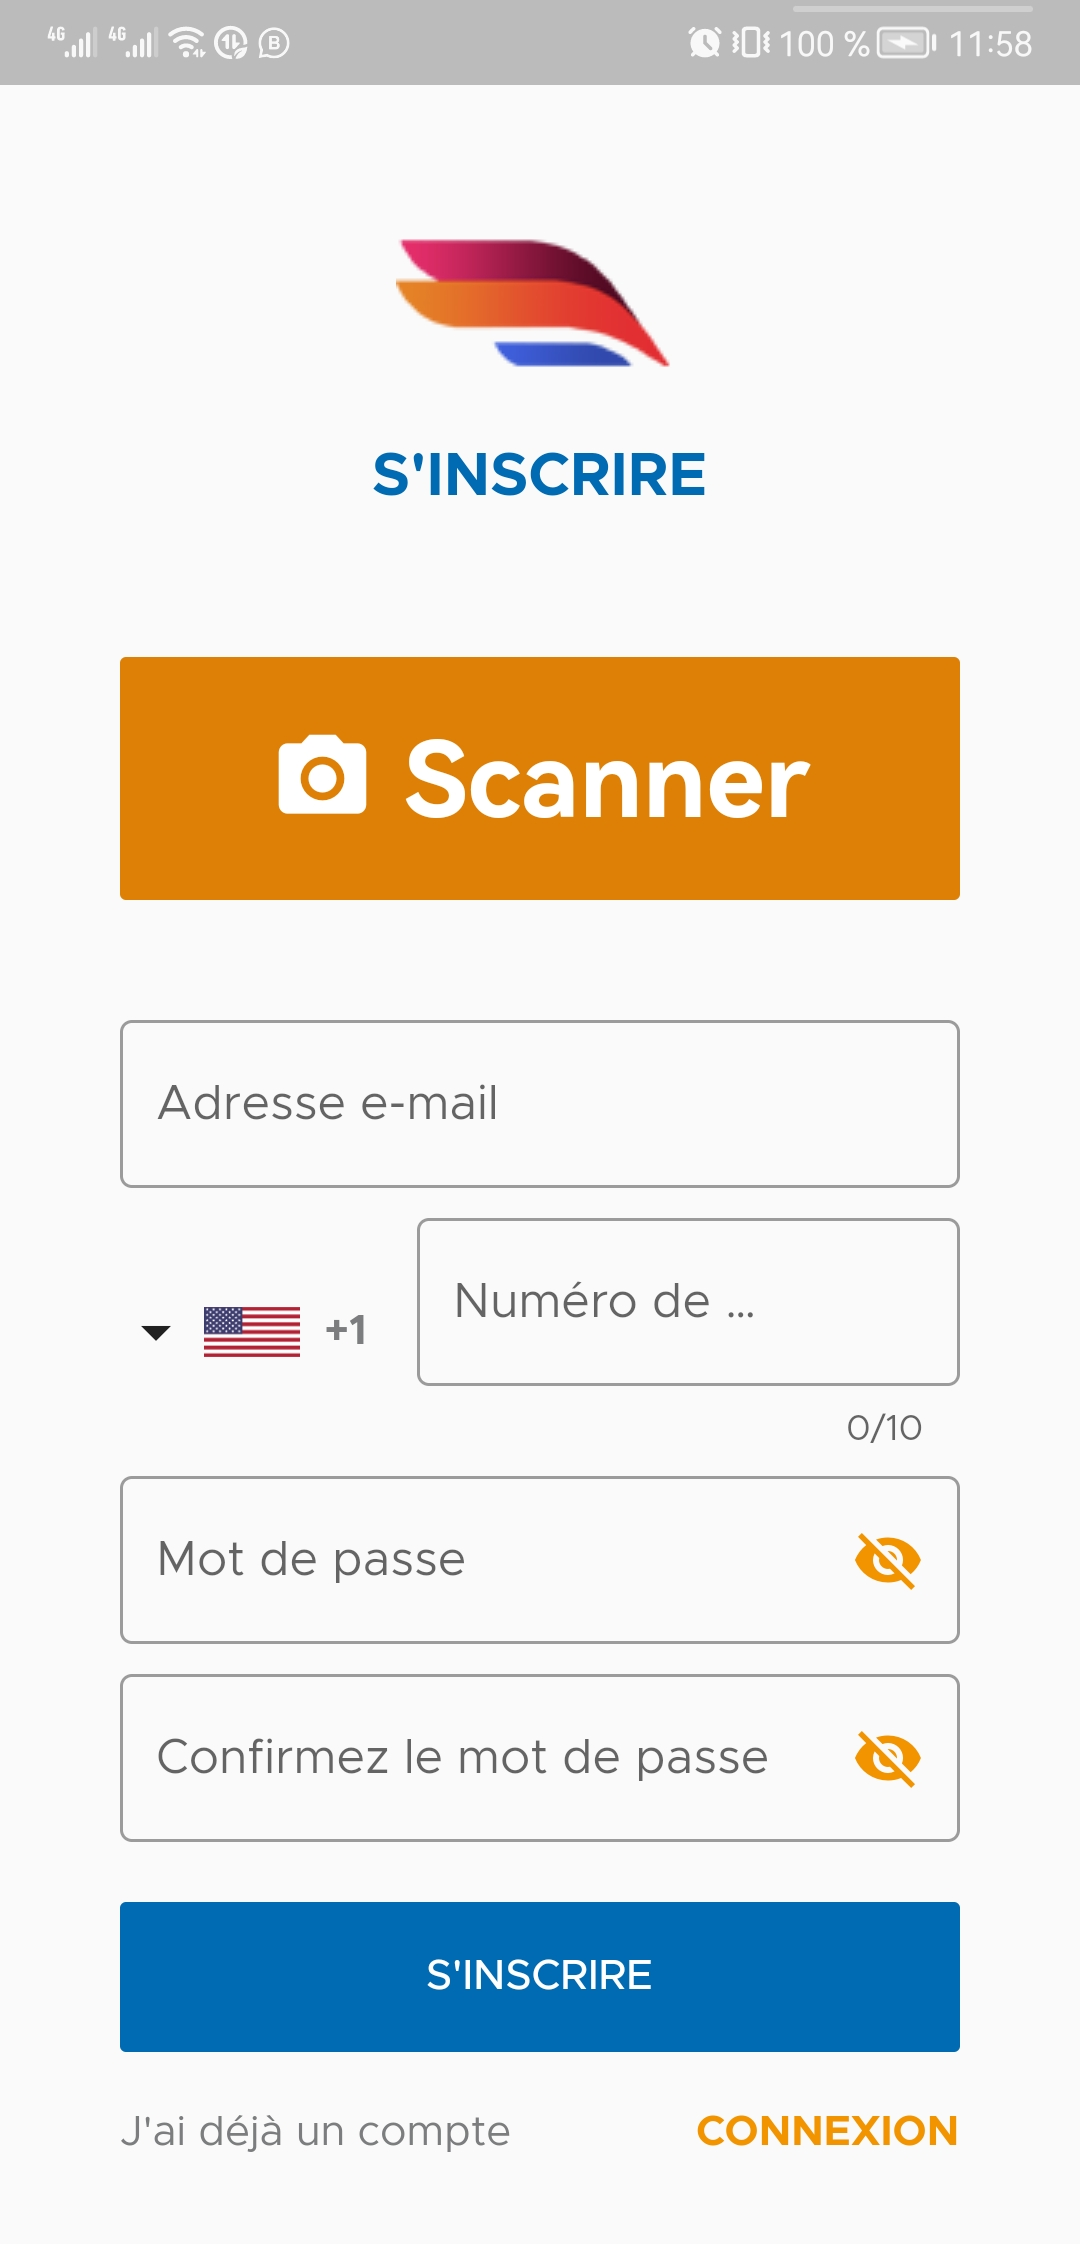
\includegraphics[scale=0.6]{D:/NTFS 3/Mon_master/M2/S4/Caputures_d_ecran_de_l_application/4}
	\includegraphics[scale=0.6]{D:/NTFS 3/Mon_master/M2/S4/Caputures_d_ecran_de_l_application/Capture}
	\centering
	\caption{Choix de génération et génération d’un nouveau Key Store.}
	\label{Figure 7.1}
\end{figure}
\newline Une fois cliqué sur \textbf{Ok}, vous aurez l’interface \ref{Figure 7.2} qui présente un aperçu sur l’ensemble des informations précédemment saisies.
\begin{figure}[!ht]
	\includegraphics[scale=0.7]{D:/NTFS 3/Mon_master/M2/S4/Caputures_d_ecran_de_l_application/2}
	\centering
	\caption{Aperçu sur la configuration de l’APK ou de l'App Bundle.}
	\label{Figure 7.2}
\end{figure}
\newline Lorsque vous cliquez sur Next, vous aurez l’interface ci-dessous. Sélectionnez le mode release, puis cliquez sur Finish. La figure \ref{Figure 7.3} en présente une illustration.
\begin{figure}[!ht]
	\includegraphics[scale=0.7]{D:/NTFS 3/Mon_master/M2/S4/Caputures_d_ecran_de_l_application/3}
	\centering
	\caption{Options de génération de l'App Bundle ou de l’APK en mode release.}
	\label{Figure 7.3}
\end{figure}
\newline Le processus de génération de l'App Bundle ou de l’APK peut durer quelques minutes suivant la performance de votre ordinateur. Une fois achevé, vous serez notifiez à ce propos. L'App Bundle ou l’APK généré en mode release se trouve dans /android/app/release du dossier du projet.
	\chapter{Annexe 2 : Déploiement des Web API et de Base de données sur Azure}
\label{chap:annexe2}

Après avoir créer un compte Azure sur \href{https://portal.azure.com/}{https://portal.azure.com/}, commencez par créer une nouvelle base de données en cliquant sur \textbf{Base de données} dans le menu à gauche puis sur \textbf{Créer}, ce qui nécessite de sélectionnez un \textbf{Groupe de ressources} \footnote{Un groupe de ressources est un conteneur regroupant les applications web et les base de données} déjà existant ou en créer un nouveau. La création de la base de données nécessite également la création d'un nouveau serveur de base de données à partir duquel vous pouvez accéder à celle-ci. Enfin, réglez les paramètres de pare-feu et votre base de donnez sera prête. Les figures \ref{Figure 8.1} expliquent le processus.
\begin{figure}[!ht]
	\includegraphics[scale=0.17]{D:/NTFS 3/Mon_master/M2/S4/Azure/Capture}
	\includegraphics[scale=0.17]{D:/NTFS 3/Mon_master/M2/S4/Azure/Capture2}
	\includegraphics[scale=0.17]{D:/NTFS 3/Mon_master/M2/S4/Azure/Capture3}
	\includegraphics[scale=0.17]{D:/NTFS 3/Mon_master/M2/S4/Azure/Capture4}
	\includegraphics[scale=0.17]{D:/NTFS 3/Mon_master/M2/S4/Azure/Capture5}
	\centering
	\caption{Création d'une base de données sur Azure.}
	\label{Figure 8.1}
\end{figure}
\newline Juste après la creation de votre base de données, Azure vous générera le chaîne de connexion (Connection String) pour que votre projet ASP .NET \footnote{Le projet ASP .NET représente les web api} pouvoir connecter à celle-ci. Voir la figure \ref{Figure 8.2}.
\begin{figure}[!ht]
	\includegraphics[scale=0.37]{D:/NTFS 3/Mon_master/M2/S4/Azure/Capture6}
	\centering
	\caption{Génération du chaîne de connexion.}
	\label{Figure 8.2}
\end{figure}
\newline Pour déployer votre web api sur Azure, vous devez créer une nouvelle application web (Web App) en cliquant sur \textbf{App Services} dans le menu à gauche puis sur \textbf{Créer}. En suite sélectionnez le même groupe de ressources que celle créé lors de la création de votre base de données puis renseignez les informations demandées, une fois terminé cliquez sur \textbf{Vérifier + créer}. Enfin, sélectionnez le niveau de tarif, puis cliquez sur \textbf{Appliquer}. Voir les figures \ref{Figure 8.3}.
\begin{figure}[!ht]
	\includegraphics[scale=0.25]{D:/NTFS 3/Mon_master/M2/S4/Azure/Capture7}
	\includegraphics[scale=0.25]{D:/NTFS 3/Mon_master/M2/S4/Azure/Capture8}
	\includegraphics[scale=0.25]{D:/NTFS 3/Mon_master/M2/S4/Azure/Capture9}
	\centering
	\caption{Creation de l'application web.}
	\label{Figure 8.3}
\end{figure}
	\chapter{Annexe 3 : Publication d’application sur Google Play Store}
\label{chap:annexe3}

Après avoir créer un compte Google Play sur \href{https://play.google.com/console/}{https://play.google.com/console/}, cliquez sur \textbf{Create app} à droite de l'écran pour créer une nouvelle application puis renseignez les informations demandées et cliquez sur \textbf{Create app} en bas de l'écran. Ensuite, cliquez sur \textbf{Main store listing} dans le menu à gauche, puis renseignez les informations demandées et cliquez sur \textbf{Save}. Ensuite, cliquez sur \textbf{Production} dans le menu à gauche aussi, puis charger l'\gls{AAB} de votre application \footnote{Google ne n'accepte plus du format APK sur le Play Store. Pour en savoir plus, veillez visiter le lien \href{https://www.phonandroid.com/tout-savoir-sur-format-aab-android-app-bundles-google-play-store.html}{https://www.phonandroid.com/tout-savoir-sur-format-aab-android-app-bundles-google-play-store.html}}, puis renseignez les informations demandées. Une fois terminé, cliquez sur \textbf{Start rollout to Production}. Les figures \ref{Figure 9.1}, \ref{Figure 9.2} et \ref{Figure 9.3} expliquent toutes les étapes à suivre.
\begin{figure}[!ht]
	\includegraphics[scale=0.3]{D:/NTFS 3/Mon_master/M2/S4/Azure/screen}
	\includegraphics[scale=0.3]{D:/NTFS 3/Mon_master/M2/S4/Azure/Capture10}
	\centering
	\caption{Publication sur Google Play Store.}
	\label{Figure 9.1}
\end{figure}
\begin{figure}[!ht]
	\includegraphics[scale=0.25]{D:/NTFS 3/Mon_master/M2/S4/Azure/Capture14}
	\includegraphics[scale=0.25]{D:/NTFS 3/Mon_master/M2/S4/Azure/Capture15}
	\includegraphics[scale=0.25]{D:/NTFS 3/Mon_master/M2/S4/Azure/Capture16}
	\includegraphics[scale=0.25]{D:/NTFS 3/Mon_master/M2/S4/Azure/Capture17}
	\centering
	\caption{Publication sur Google Play Store 2.}
	\label{Figure 9.2}
\end{figure}
\begin{figure}[!ht]
	\includegraphics[scale=0.25]{D:/NTFS 3/Mon_master/M2/S4/Azure/Capture14}
	\includegraphics[scale=0.25]{D:/NTFS 3/Mon_master/M2/S4/Azure/Capture15}
	\includegraphics[scale=0.25]{D:/NTFS 3/Mon_master/M2/S4/Azure/Capture16}
	\includegraphics[scale=0.25]{D:/NTFS 3/Mon_master/M2/S4/Azure/Capture17}
	\centering
	\caption{Publication sur Google Play Store 3.}
	\label{Figure 9.3}
\end{figure}	
	
	
	\let\cleardoublepage\clearpage
	
	\chapter*{Bibliographie}
	\addcontentsline{toc}{chapter}{Bibliographie}
	\chaptermark{Références}
	\printbibliography[heading=none]
	
	\begin{enumerate}
		\item \bibliography{Véronique Messager Rota, Gestion de projet vers les méthodes agiles.}
		
		\item 	\bibliography{Rivest, Ronald L (1990), « The MD4 message digest algorithm », in : Conference on the Theory and
			Application of Cryptography, Springer, p. 303–311.}
		
		\item \bibliography{Rivest, Ronald et S Dusse (1992), The MD5 message-digest algorithm.}
		
		\item \bibliography{Anderson, Ross et Eli Biham (1996), « Tiger : A fast new hash function », in : International Workshop
			on Fast Software Encryption, Springer, p. 89–97.}
		
		\item 	\bibliography{Dobbertin, Hans, Antoon Bosselaers et Bart Preneel (1996), « RIPEMD-160 : A strengthened
			version of RIPEMD », in : International Workshop on Fast Software Encryption, Springer, p. 71–
			82.}
		
		\item \bibliography{Barreto, PSLM, Vincent Rijmen et al. (2000), « The Whirlpool hashing function », in : First open
			NESSIE Workshop, Leuven, Belgium, t. 13, p. 14.}
		
		\item \bibliography{Rivest, Ronald L et al. (2008), « The MD6 hash function–a proposal to NIST for SHA-3 », in :
			Submission to NIST 2.3, p. 1–234.}
		
		\item \bibliography{Aumasson, Jean-Philippe et al. (2008), « Sha-3 proposal blake », in : Submission to NIST 92.}
		
		\item \bibliography{Michail, Haralambos et al. (2005), « A low-power and high-throughput implementation of the SHA-1
			hash function », in : 2005 IEEE International Symposium on Circuits and Systems, IEEE, p. 4086–
			4089.}
		
		\item \bibliography{Glabb, Ryan et al. (2007), « Multi-mode operator for SHA-2 hash functions », in : journal of systems
			architecture 53.2-3, p. 127–138.}
		
		\item \bibliography{Dworkin, Morris J (2015), SHA-3 standard : Permutation-based hash and extendable-output functions,
			rapp. tech.}
		
		\item 	\bibliography{Dolmatov, Vasily et Alexey Degtyarev (2013), « GOST R 34.11-2012 : hash function », in : Independent
			Submission, Ed. Request for Comments : Updates 5831, p. 2070–1721.}
	\end{enumerate}
	
	

\end{document}